\documentclass[
	% -- opções da classe memoir --
	12pt,				% tamanho da fonte
	openright,			% capítulos começam em pág ímpar (insere página vazia caso preciso)
	oneside,			% para impressão em recto e verso. Oposto a oneside
	a4paper,			% tamanho do papel. 
	% -- opções da classe abntex2 --
	%chapter=TITLE,		% títulos de capítulos convertidos em letras maiúsculas
	%section=TITLE,		% títulos de seções convertidos em letras maiúsculas
	%subsection=TITLE,	% títulos de subseções convertidos em letras maiúsculas
	%subsubsection=TITLE,% títulos de subsubseções convertidos em letras maiúsculas
	% -- opções do pacote babel --
	english,			% idioma adicional para hifenização
	brazil				% o último idioma é o principal do documento
	]{abntex2}

% Pacotes básicos 
\usepackage{lmodern}			% Usa a fonte Latin Modern			
\usepackage[T1]{fontenc}		% Selecao de codigos de fonte.
\usepackage[utf8]{inputenc}		% Codificacao do documento (conversão automática dos acentos)
\usepackage{indentfirst}		% Indenta o primeiro parágrafo de cada seção.
\usepackage{color}			% Controle das cores
\usepackage{graphicx}			% Inclusão de gráficos
\usepackage{microtype} 			% para melhorias de justificação

% Pacotes adicionais, usados apenas no âmbito do Modelo Canônico do abnteX2
\usepackage{amsmath}
\usepackage{amsthm,amsfonts}
\usepackage[list=true,listformat=simple]{subcaption}

% Pacotes de citações
\usepackage[brazilian,hyperpageref]{backref}	% Paginas com as citações na bibl
\usepackage[alf]{abntex2cite}			% Citações padrão ABNT
\usepackage{listings}				% Ambiente de linguagens de desenvolvimento
\usepackage{xcolor}
\definecolor{commentgreen}{RGB}{2,112,10}
\definecolor{weborange}{RGB}{255,165,0}
\lstset {
    language=Matlab,
    frame=tb,
    tabsize=4,
    showstringspaces=false,
    numbers=left,
    %upquote=true,
    commentstyle=\color{commentgreen},
    basicstyle=\small\ttfamily, % basic font setting
    emph={int,char,double,float,unsigned,void,bool},
    emphstyle={\color{blue}},
    escapechar=\&,
    % keyword highlighting
    classoffset=1, % starting new class
    otherkeywords={>,<,.,;,-,!,=,~},
    morekeywords={>,<,.,;,-,!,=,~},
    keywordstyle=\color{weborange},
    classoffset=0,
}


% CONFIGURAÇÕES DE PACOTES

% Configurações do pacote backref
% Usado sem a opção hyperpageref de backref
\renewcommand{\backrefpagesname}{Citado na(s) página(s):~}
% Texto padrão antes do número das páginas
\renewcommand{\backref}{}
% Define os textos da citação
\renewcommand*{\backrefalt}[4]{
	\ifcase #1 %
		Nenhuma citação no texto.%
	\or
		Citado na página #2.%
	\else
		Citado #1 vezes nas páginas #2.%
	\fi}%

% Informações de dados para CAPA e FOLHA DE ROSTO
\titulo{Implementação de técnica de controle em um manipulador robótico utilizando o 
conceito de \textit{Hardware in the Loop}}
\autor{Luiz Henrique Silva Lelis}
\local{Belo Horizonte}
\data{2019, v1}
\orientador{Luciano Antonio Frezzatto Santos}
%\coorientador{Equipe \abnTeX}
\instituicao{%
  Universidade Federal de Minas Gerais -- UFMG
  \par
  Escola de Engenharia}
\tipotrabalho{Trabalho de Conclusão de Curso}
% O preambulo deve conter o tipo do trabalho, o objetivo, 
% o nome da instituição e a área de concentração 
\preambulo{Trabalho de Conclusão de Curso apresentado à Universidade Federal de 
Minas Gerais para obtenção do Título de Bacharel em Engenharia de Controle e Automação
pela Escola de Engenharia da Universidade Federal de Minas Gerais.}

% Configurações de aparência do PDF final
% alterando o aspecto da cor azul
\definecolor{blue}{RGB}{41,5,195}

% informações do PDF
\makeatletter
\hypersetup{
  %pagebackref=true,
  pdftitle={\@title}, 
  pdfauthor={\@author},
  pdfsubject={\imprimirpreambulo},
  pdfcreator={LaTeX with abnTeX2},
  pdfkeywords={hardware-in-the-loop, }{manipulador robótico, }{trabalho acadêmico}, 
  colorlinks=true,       		% false: boxed links; true: colored links
  linkcolor=black,          	% color of internal links
  citecolor=black,        		% color of links to bibliography
  filecolor=magenta,      		% color of file links
  urlcolor=black,
  bookmarksdepth=4
}
\makeatother

% Posiciona figuras e tabelas no topo da página quando adicionadas sozinhas
% em um página em branco. Ver https://github.com/abntex/abntex2/issues/170
\makeatletter
\setlength{\@fptop}{5pt} % Set distance from top of page to first float
\makeatother

% Possibilita criação de Quadros e Lista de quadros.
% Ver https://github.com/abntex/abntex2/issues/176
\newcommand{\quadroname}{Quadro}
\newcommand{\listofquadrosname}{Lista de quadros}
\renewcommand{\sin}{\mathrm{sen}}
\newcommand{\refanexo}[1]{\hyperref[#1]{Anexo~\ref{#1}}}

\newfloat[chapter]{quadro}{loq}{\quadroname}
\newlistof{listofquadros}{loq}{\listofquadrosname}
\newlistentry{quadro}{loq}{0}

% configurações para atender às regras da ABNT
\setfloatadjustment{quadro}{\centering}
\counterwithout{quadro}{chapter}
\renewcommand{\cftquadroname}{\quadroname\space} 
\renewcommand*{\cftquadroaftersnum}{\hfill--\hfill}

\setfloatlocations{quadro}{hbtp} % Ver https://github.com/abntex/abntex2/issues/176

% Espaçamentos entre linhas e parágrafos 

% O tamanho do parágrafo é dado por:
\setlength{\parindent}{1.3cm}

% Controle do espaçamento entre um parágrafo e outro:
\setlength{\parskip}{0.2cm}  % tente também \onelineskip

% compila o indice
\makeindex

% Início do documento
\begin{document}

% Seleciona o idioma do documento (conforme pacotes do babel)
%\selectlanguage{english}
\selectlanguage{brazil}

% Retira espaço extra obsoleto entre as frases.
\frenchspacing 

% ----------------------------------------------------------
% ELEMENTOS PRÉ-TEXTUAIS
% ----------------------------------------------------------
% \pretextual
\pagenumbering{arabic}
\setcounter{page}{1}

% Capa
\imprimircapa

% Folha de rosto
\imprimirfolhaderosto*

% Inserir a ficha bibliografica
% \begin{fichacatalografica}
%     \includepdf{fig_ficha_catalografica.pdf}
% \end{fichacatalografica}
%\begin{fichacatalografica}
	\sffamily
	\vspace*{\fill}					% Posição vertical
	\begin{center}					% Minipage Centralizado
	\fbox{\begin{minipage}[c][8cm]{13.5cm}		% Largura
	\small
	\imprimirautor
	%Sobrenome, Nome do autor
	
	\hspace{0.5cm} \imprimirtitulo  / \imprimirautor. --
	\imprimirlocal, \imprimirdata-
	
	\hspace{0.5cm} \thelastpage p. : il. (algumas color.) ; 30 cm.\\
	
	\hspace{0.5cm} \imprimirorientadorRotulo~\imprimirorientador\\
	
	\hspace{0.5cm}
	\parbox[t]{\textwidth}{\imprimirtipotrabalho~--~\imprimirinstituicao,
	\imprimirdata.}\\
	
	\hspace{0.5cm}
	\textit{hardware-in-the-loop}}{controle}{manipulador robótico}
  {trabalho acadêmico}
		1. \textit{hardware in the loop}.
		2. Palavra-chave2.
		3. Palavra-chave3.
		I. \imprimirorientador.
		II. Universidade Federal de Minas Gerais.
		III. Escola de Engenharia.
		IV. \imprimirtitulo. 			
	\end{minipage}}
	\end{center}
\end{fichacatalografica}

% Inserir errata
%\begin{errata}
Elemento opcional da \citeonline[4.2.1.2]{NBR14724:2011}. Exemplo:

\vspace{\onelineskip}

FERRIGNO, C. R. A. \textbf{Tratamento de neoplasias ósseas apendiculares com
reimplantação de enxerto ósseo autólogo autoclavado associado ao plasma
rico em plaquetas}: estudo crítico na cirurgia de preservação de membro em
cães. 2011. 128 f. Tese (Livre-Docência) - Faculdade de Medicina Veterinária e
Zootecnia, Universidade de São Paulo, São Paulo, 2011.

\begin{table}[htb]
\center
\footnotesize
\begin{tabular}{|p{1.4cm}|p{1cm}|p{3cm}|p{3cm}|}
  \hline
   \textbf{Folha} & \textbf{Linha}  & \textbf{Onde se lê}  & \textbf{Leia-se}  \\
    \hline
    1 & 10 & auto-conclavo & autoconclavo\\
   \hline
\end{tabular}
\end{table}

\end{errata}

% Inserir folha de aprovação
% \begin{folhadeaprovacao}
% \includepdf{folhadeaprovacao_final.pdf}
% \end{folhadeaprovacao}
%\begin{folhadeaprovacao}

  \begin{center}
    {\ABNTEXchapterfont\large\imprimirautor}

    \vspace*{\fill}\vspace*{\fill}
    \begin{center}
      \ABNTEXchapterfont\bfseries\Large\imprimirtitulo
    \end{center}
    \vspace*{\fill}
    
    \hspace{.45\textwidth}
    \begin{minipage}{.5\textwidth}
        \imprimirpreambulo
    \end{minipage}%
    \vspace*{\fill}
   \end{center}
        
   Trabalho aprovado. \imprimirlocal, 24 de novembro de 2012:

   \assinatura{\textbf{\imprimirorientador} \\ Orientador} 
   \assinatura{\textbf{Professor} \\ Convidado 1}
   \assinatura{\textbf{Professor} \\ Convidado 2}
   %\assinatura{\textbf{Professor} \\ Convidado 3}
   %\assinatura{\textbf{Professor} \\ Convidado 4}
      
   \begin{center}
    \vspace*{0.5cm}
    {\large\imprimirlocal}
    \par
    {\large\imprimirdata}
    \vspace*{1cm}
  \end{center}
  
\end{folhadeaprovacao}

% Dedicatória
%\begin{dedicatoria}
   \vspace*{\fill}
   \centering
   \noindent
   \textit{ Este trabalho é dedicado às crianças adultas que,\\
   quando pequenas, sonharam em se tornar cientistas.} \vspace*{\fill}
\end{dedicatoria}

% Agradecimentos
%\begin{agradecimentos}
Os agradecimentos principais são direcionados à Gerald Weber, Miguel Frasson,
Leslie H. Watter, Bruno Parente Lima, Flávio de Vasconcellos Corrêa, Otavio Real
Salvador, Renato Machnievscz\footnote{Os nomes dos integrantes do primeiro
projeto abn\TeX\ foram extraídos de
\url{http://codigolivre.org.br/projects/abntex/}} e todos aqueles que
contribuíram para que a produção de trabalhos acadêmicos conforme
as normas ABNT com \LaTeX\ fosse possível.

Agradecimentos especiais são direcionados ao Centro de Pesquisa em Arquitetura
da Informação\footnote{\url{http://www.cpai.unb.br/}} da Universidade de
Brasília (CPAI), ao grupo de usuários
\emph{latex-br}\footnote{\url{http://groups.google.com/group/latex-br}} e aos
novos voluntários do grupo
\emph{\abnTeX}\footnote{\url{http://groups.google.com/group/abntex2} e
\url{http://www.abntex.net.br/}}~que contribuíram e que ainda
contribuirão para a evolução do \abnTeX.
\end{agradecimentos}

% Epigrafe
%\begin{epigrafe}
    \vspace*{\fill}
	\begin{flushright}
		\textit{``Não vos amoldeis às estruturas deste mundo, \\
		mas transformai-vos pela renovação da mente, \\
		a fim de distinguir qual é a vontade de Deus: \\
		o que é bom, o que Lhe é agradável, o que é perfeito.\\
		(Bíblia Sagrada, Romanos 12, 2)}
	\end{flushright}
\end{epigrafe}

% resumo em português
%\setlength{\absparsep}{18pt} % ajusta o espaçamento dos parágrafos do resumo
\begin{resumo}
  A técnica \textit{Hardware in the Loop} (HIL) é fundamental para simulações em tempo real a fim de conectar uma parte 
  do sistema a um modelo digital. A técnica consiste na inserção de um dispositivo físico na malha de controle
  durante o desenvolvimento do sistema. Atualmente, as simulações HIL são utilizadas principalmente para o 
  desenvolvimento de novos componentes e atuadores em vários campos diferentes como: simulações de voo, 
  sistemas eletrônicos de potência, robótica móvel e engenharia de tráfego. No sistema estudado nesta monografia, a técnica 
  HIL é aplicada a um manipulador robótico simplificado com três juntas de revolução. O método foi aplicado em 
  três etapas distintas: a primeira consiste no levantamento do modelo da planta e sintonia do controlador em 
  ambiente de simulação; a segunda na substituição do controlador virtual por sua implementação em dispositivo 
  físico seguido da validação em conjunto com o ambiente de simulação; por fim, a última etapa corresponde à 
  utilização do controlador implementado no dispositivo físico comunicando diretamente com a planta real. O projeto
  faz uso do computador de placa única \textit{Raspberry Pi} como o Hardware inserido na malha de controle do manipulador.
  Finalmente, destaca-se como objetivo do projeto a sintonia e validação do controle de juntas independentes do
  manipulador em questão aplicando a técnica HIL.
  
 \textbf{Palavras-chave}: \textit{Hardware in the Loop}, manipulador robótico, controle, juntas independentes.
\end{resumo}

% resumo em inglês
%\begin{resumo}[Abstract]
 \begin{otherlanguage*}{english}
  The Hardware in the Loop (HIL) technique is fundamental for real-time simulations in order to connect
  a part of the system to a digital model. The technique consists in the insertion of a physical device in
  the control loop during the system's development. Currently, HIL simulations are mainly used for the 
  development of new components and actuators in several fields such as: flight simulations, 
  electronic power systems, mobile robotics and traffic engineering. For the system studied in this monography, the HIL
  technique is applied to a simplified robotic manipulator with three revolute joints. The method was
  applied in three distinct steps: the first one consists in surveying the plant model and tuning the
  controller in a simulation environment; the second is the replacement of the virtual controller by
  its implementation in a physical device followed by the validation within the simulation environment;
  finally, the last step corresponds to the use of the controller implemented in the physical device
  communicating directly with the actual plant. The project makes use of the single board computer 
  Raspberry Pi as the hardware inserted into the loop of the manipulator's control. Finally, an independent
  joint control for the manipulator applying, applying the HIL technique.

  \vspace{\onelineskip}
 
   \noindent 
   \textbf{Keywords}: Hardware in the Loop, robotic manipulator, control, independent joints.
 \end{otherlanguage*}
\end{resumo}

% inserir lista de ilustrações
\pdfbookmark[0]{\listfigurename}{lof}
\listoffigures*
\cleardoublepage

% inserir lista de quadros
%\pdfbookmark[0]{\listofquadrosname}{loq}
%\listofquadros*
%\cleardoublepage

% inserir lista de tabelas
%\pdfbookmark[0]{\listtablename}{lot}
%\listoftables*
%\cleardoublepage

% inserir lista de abreviaturas e siglas
%\begin{siglas}
  \item[DH] \textit{Denavit-Hartenberg}
  \item[DOF] \textit{Degree-of-freedom}
  \item[EL] \textit{Euler-Lagrange}
  \item[HIL] \textit{Hardware in the Loop}
  \item[MA] Malha aberta
  \item[MF] Malha fechada
  \item[PI] Proporcional Integral
  \item[PID] Proporcional Integral Derivativo
  \item[PPP] Prismática Prismática Prismática
  \item[RPP] Rotacional Prismática Prismática
  \item[RRP] Rotacional Rotacional Prismática
  \item[RRR] Rotacional Rotacional Rotacional
  \item[SCARA] \textit{Selective Compliance Assembly Robot Arm}
  \item[UART] \textit{Universal Asynchrounous Receiver/Transmiter}
\end{siglas}

% inserir lista de símbolos
%\begin{simbolos}
	\item[$ \ddot{q}_n $] 	aceleração generalizada da junta $n$
	\item[$ \theta_i $] 	ângulo da junta $i$
	\item[$\xi$]		coeficiente de amortecimento
	\item[$ r_{ci} $]	coordenada do centro de massa do elo $i$
	\item[$ g $]		constante de gravidade
	\item[$\tau$]		constante de tempo do sistema de primeira ordem
	\item[$ \rho $]		densidade de massa
	\item[$ d_i $]		deslocamento do elo
	\item[$ d_{kj} $]	elemento da matriz $D(q)$
	\item[$ d_{ki} $]	elemento da matriz $D(q)$
	\item[$ d_{ij} $]	elemento da matriz $D(q)$
	\item[$ c_{ijk} $]	elemento da matriz de Coriolis
	\item[$ \phi_k $]	elemento da matriz $g(q)$ obtido da energia potencial, relativo à força generalizada aplicada $k$
	\item[$ K $]		energia cinética
	\item[$ P $]		energia potencial
	\item[$ P_i $]		energia potencial do elo $i$
	\item[$\omega_n$]	frequência natural não amortecida
	\item[$ \tau_i $]	força generalizada aplicada na junta $i$
	\item[$K_p$]		ganho proporcional
	\item[$ \alpha_i $]	giro do elo
	\item[$ J_i $]		Jacobiano da junta $i$
	\item[$ J_{\omega} $]	Jacobiano relativo à velocidade angular
	\item[$ J_v $]		Jacobiano relativo à velocidade linear
	\item[$ m_i $]		massa do elo $i$
	\item[$ D(q) $]		matriz da equação dinâmica que incorpora a energia cinética do manipulador
	\item[$ \zeta $]	matriz das velocidades linear e angular
	\item[$ I $]		matriz de inércia
	\item[$ R $]		matriz de rotação
	\item[$ R_n^0 $]	matriz de rotação do elo $n$ em relação à base
	\item[$ A_i $]		matriz de transformação homogênea do elo $i$
	\item[$ T_n^0 $]	matriz de transformação homogênea do elo $n$ em relação à base
	\item[$ o_n^0 $]	matriz de translação do órgão terminal em relação à base $C(q, q)$
	\item[$ C(q,\dot{q}) $]	matriz que incorpora os símbolos de Christoffel
	\item[$ g(q) $]		matriz que incorpora a energia potencial do manipulador
	\item[$ I_{xx} $]	momento principal de inércia sobre o eixo $x$
	\item[$ I_{yy} $]	momento principal de inércia sobre o eixo $y$
	\item[$ I_{zz} $]	momento principal de inércia sobre o eixo $z$
	\item[$ I_{xy} $]	produto cruzado de inércia dos eixos $x$ e $y$
	\item[$ I_{xz} $]	produto cruzado de inércia dos eixos $x$ e $z$
	\item[$ I_{yx} $]	produto cruzado de inércia dos eixos $y$ e $x$
	\item[$ I_{yz} $]	produto cruzado de inércia dos eixos $y$ e $z$
	\item[$ I_{zx} $]	produto cruzado de inércia dos eixos $z$ e $x$
	\item[$ I_{zy} $]	produto cruzado de inércia dos eixos $z$ e $y$
	\item[$ a_i $]		tamanho do elo
	\item[$T_d$]		tempo derivativo
	\item[$T_i$]		tempo integral
	\item[$ \Gamma $]	tensor de inércia
	\item[$ q_n $]		variável generalizada da junta $n$
	\item[$ \omega $]	velocidade angular
	\item[$ \omega_n^0 $]	velocidade angular do elo $n$ em relação à base
	\item[$ \dot{q}_n $]	velocidade generalizada da junta $n$
	\item[$ v $]		velocidade linear
	\item[$ v_n^0 $]	velocidade linear do elo $n$ em relação à base
\end{simbolos}

% inserir o sumario
\pdfbookmark[0]{\contentsname}{toc}
\tableofcontents*
\cleardoublepage

% ----------------------------------------------------------
% ELEMENTOS TEXTUAIS
% ----------------------------------------------------------
\textual

%\pagenumbering{arabic}
\chapter{Introdução}
%\markboth{\thechapter ~~~ Introdução}{}
%\label{intro}

Um sistema pode ser visto como um processo com sinais de entrada que são 
transformados ou induzidos a responder de alguma forma, resultando em outros 
sinais de saída \cite{Oppenhein}. O intuito do controlador é manipular o sistema com a 
finalidade de obter um sinal de saída que seja desejado. A implementação do 
controlador é fundamental para tornar possível processos em diferentes áreas como 
sistemas eletrônicos de potência \cite{Rothstein}, acionamentos elétricos 
\cite{Bouscayrol}, engenharia de tráfego \cite{Bullock} e robótica móvel 
\cite{Kamali}. Para isso, os sistemas são modelados matematicamente através de 
equações diferenciais lineares, e o controlador é projetado a partir do modelo 
matemático.

No controle em malha aberta, a saída não exerce nenhuma ação sobre o sinal de 
controle. Desta forma, aplica-se um sinal na entrada de uma planta ou de um 
processo para que a variável controlada atinja um valor desejado, mas este 
valor obtido na saída não é utilizado para modificar a entrada. O problema 
deste tipo de controle é que o sistema pode adquirir novas características 
, por exemplo, ao ocorrerem perturbações. Caso isso ocorra, a saída não 
terá o valor desejado anteriormente.

Ao fechar a malha, o sinal de saída passa a interferir diretamente na ação de 
controle. Assim, o sistema ganha o conceito de realimentação e erro, 
e o controlador tende a reduzir o erro (deferença entre os valores de referência 
e realimentação) e a manter a saída no valor desejado. ``Controlar a saída de 
uma planta ou de um processo por realimentação significa aplicar na sua entrada, 
após conveniente amplificação, o sinal resultante da 
diferença entre o valor desejado e o valor medido da saída \cite[p.~3]{Castrucci}.''

A simulação \emph{Hardware in the Loop} (HIL) é uma técnica bem estabelecida 
usada em projeto e avaliação de sistemas de controle \cite{Bacic}. Esta técnica de 
controle consiste em projetar o controlador para uma determinada planta 
substituindo o bloco de controle $C(s)$ na Figura \ref{fig:diagBloco} por um 
microcontrolador físico e validando o desempenho do sistema em malha fechada com 
esse controlador, como ilustrado na Figura \ref{fig:diagBlocoHIL}.

\begin{figure}[ht]
  \centering
  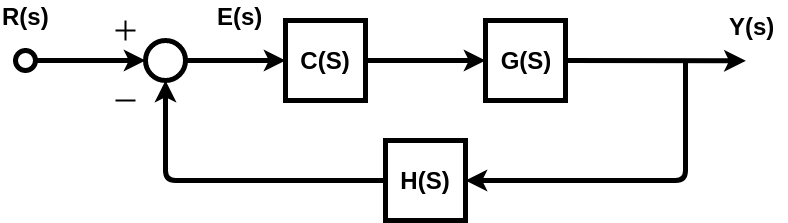
\includegraphics[width = 0.6\columnwidth]{Imagens/blocosMF.png}
  \caption{Diagrama de blocos do sistema em malha fechada}
  \label{fig:diagBloco} 
\end{figure}

\begin{figure}[ht]
  \centering
  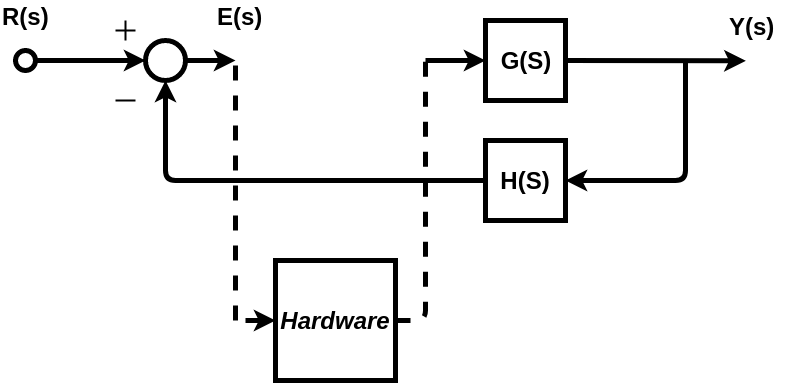
\includegraphics[width = 0.7\columnwidth]{Imagens/blocoHard.png}
  \caption{Diagrama de blocos do sistema em malha fechada - \emph{Hardware in the Loop}}
  \label{fig:diagBlocoHIL} 
\end{figure}

% O que este PFC pretende alcançar e como? Metodologia a ser seguida.

O controle em malha fechada utiliza a informação de como a variável controlada evolui 
para determinar o sinal de controle aplicado ao processo. Determinado o modelo da 
planta a ser controlada, o controlador é sintonizado de forma a atender especificações 
de projeto fornecidas. Geralmente, 
uma vez sintonizado o controlador e validado o desempenho em malha fechada da 
planta realimentada, passa-se a implementação prática do controle sem que haja 
uma prévia validação do comportamento do controlador quando implementado em 
dispositivo físico. 

O controle da planta possui três etapas distintas de execução. A primeira trata-se 
do projeto do controlador simulado em conjunto com o modelo da planta; a segunda 
é a implementação em dispositivo físico do controlador e validação com 
o modelo da planta; e a terceira trata-se da validação da estratégia de controle 
na planta física.

\section{Motivação e Justificativa}
\markright{\thesection ~~~ Motivação e Justificativa}
%\label{motiva}

Nos dias de hoje, as simulações \emph{Hardware in the Loop} (HIL) são utilizadas
cada vez mais para desenvolverem novos componentes e atuadores em vários campos
diferentes \cite{Bouscayrol}. A ação de controle agora não depende 
apenas da computação numérica, mas também da forma como o modelo interage com um 
equipamento de controle externo. Além disso, o conceito de sistemas embarcados 
exige cada vez mais o uso de ferramentas independentes encarregadas de executar 
uma função específica.

Sabe-se que os seres humanos têm limitações para frequentar determinados ambientes, 
principalmente os ambientes industriais, onde estão submetidos a alta insalubridade 
\cite{Lacaz}. Consequentemente, nos últimos anos, tem sido cada vez mais frequente 
em indústrias, o uso de tecnologias que visam automatizar seus processos de 
fabricação. Estas soluções visam a melhoria na qualidade do trabalho, e, 
consequentemente, um aumento de produtividade. Os manipuladores robóticos são 
exemplos de soluções deste tipo, sejam eles controlados remotamente, ou totalmente independentes 
da ação humana. A maior parte das aplicações de manipuladores está voltada para a indústria, 
principalmente as que utilizam linhas de produção (como montadoras e fabricantes de autopeças)
\cite{Spong}.

\section{Objetivos do Projeto}
\markright{\thesection ~~~ Objetivos do Projeto}
%label{objetivos}

O objetivo principal do presente projeto é sintonizar e validar estratégias de 
controle para o sistema dinâmico de um manipulador robótico utilizando a técnica 
\emph{Hardware in the Loop} (HIL). Além disso, será construída uma plataforma de 
validação de controladores através do \emph{Hardware in the Loop} (HIL).

\section{Local de Realização}
\markright{\thesection ~~~ Local de Realização}
%\label{empresa}

Departamento de Engenharia Eletrônica da UFMG (DELT/UFMG). O departamento 
situa-se dentro do campus Pampulha da UFMG na Escola de Engenharia. O campus 
fica na Av. Presidente Antônio Carlos 6627 - Pampulha, Belo Horizonte - MG, 
31270-901.

O departamento foi criado em 1969 e tem contribuído para a formação dos 
engenheiros eletricistas e engenheiros de controle e automação da UFMG. O DELT é 
referência no cenário nacional, e, é também, o Departamento da UFMG com maior 
participação no curso de graduação em Engenharia de Controle e Automação.

\section{Estrutura da Monografia}
\markright{\thesection ~~~ Estrutura da Monografia}
%\label{organizacao}

A monografia está dividida em cinco capítulos. Este capítulo apresentou uma introdução 
ao projeto e o local onde o trabalho foi realizado. O Capítulo 2 descreve 
os princípios básicos de um manipulador robótico e a técnica \emph{Hardware in the 
Loop} (HIL). Ele também abrange todos os conceitos necessários para um melhor 
entendimento do trabalho. O Capítulo 3 aborda a metodologia de desenvolvimento do trabalho. 
Nesse capítulo são feitas a modelagem da planta de estudo e validação do modelo, a 
concepção do ambiente de simulação, as especificações das estratégias de controle no 
microcontrolador e, por fim, as validações das estratégias por meio de simulações. 
Os resultados experimentais são apresentados no Capítulo 4. Primeiramente, a 
metodologia HIL é validada, para diferentes estratégias de controle, no ambiente 
de simulação concebido no Capítulo 3 e, posteriormente, os controladores 
implementados são aplicados à planta física em estudo. 
Finalmente, no capítulo 5, tem-se a conclusão da  monografia com algumas sugestões 
para trabalhos futuros e dificuldades encontradas na realização do projeto.


\clearpage
\chapter{Revisão Bibliográfica}
%\markboth{\thechapter ~~~ Revisão Bibliográfica}{}
%\label{revBib}

Esta monografia pretende validar estratégias de controle em um manipulador robótico 
por meio da técnica \textit{Hardware in the Loop} (HIL). Por esse motivo, este capítulo 
aborda uma breve revisão dos principais aspectos que envolvem o tema proposto: manipuladores 
robóticos, sistemas de controle e HIL. Por clareza, esses tópicos são apresentados em seções 
distintas.


\section{Manipuladores Robóticos}
\markright{\thesection ~~~ Manipuladores Robóticos}
%\label{manipRob}

Um manipulador robótico pode ser definido como um mecanismo reprogramável e multifuncional
que é desenvolvido para mover materiais, peças e ferramentas \cite{Murphy:2000:IAR:517685}. 
Mecanismo este que é composto por elos e juntas mecânicas. Apesar disso, o manipulador não pode ser 
visto apenas como uma série de elos (ou \textit{links}) em cascata. Para \citeonline{Spong}, 
o manipulador robótico é composto por um braço mecânico, pela ferramenta no fim do braço 
(também chamada ferramenta de trabalho), pela fonte de energia externa, pelos sensores 
externos e internos, pela interface de comunicação com o sistema e pelo controle do microcontrolador.

Na construção do manipulador, os elos são conectados por meio de juntas formando a cadeia 
cinemática. Segundo \citeonline{paul1981robot}, ao incorporar coordenadas em cada elo do manipulador, 
usando transformação homogênea, é possível descrever a posição relativa e a orientação entre elas.
A transformação homogênea corresponde a transformação de coordenadas que descreve a posição e a orientação 
do eixo da ferramenta de trabalho em relação à base (eixo $0$) \cite{siciliano}.

As juntas podem ser tanto de revolução quanto prismáticas \cite{paul1981robot}. As juntas de revolução
são aquelas que permitem um movimento de rotação entre um elo e outro. Por outro lado,
as prismáticas são as que possibilitam apenas um movimento linear entre os elos.

A forma geométrica para se classificar os manipuladores é dada pela disposição das juntas 
na cadeia cinemática. Segundo \citeonline{Spong}, a maioria dos manipuladores se 
enquadra em uma das categorias a seguir (em que R corresponde a uma junta de revolução 
e P uma junta prismática): articulada (RRR), esférica (RRP), SCARA (RRP), cilíndrica 
(RPP), ou Cartesiana (PPP).

O grau de liberdade (DOF - \textit{degree-of-freedom}) é um parâmetro fundamental para 
a configuração espacial do manipulador robótico. É esse parâmetro que define qual a dimensão do 
espaço de configuração, ou seja, um manipulador possui \textit{n} graus de liberdade caso sua 
configuração seja minimamente especificada por \textit{n} parâmetros \cite{Spong}. Para 
\citeonline{Spong}, a maioria dos manipuladores industriais atualmente possuem seis 
ou menos graus de liberdade.

É importante ressaltar que a planta utilizada neste trabalho é um manipulador com três juntas
revolutas. O manipulador real, possui outras duas juntas, uma para o punho e outra para a garra, entretanto estas 
foram desconsideradas para a modelagem e para o controle. Esse manipulador está representado na \autoref{fig:manipuladorRRR} e 
também é conhecido na literatura como manipulador de cotovelos (\textit{elbow manipulator}), articulado, revoluto, 
antropomórfico (\textit{anthropomorphic manipulator}) ou manipulador RRR.

\begin{figure}[ht]
  \centering
  \caption{Planta utilizada - manipulador de três juntas revolutas}
  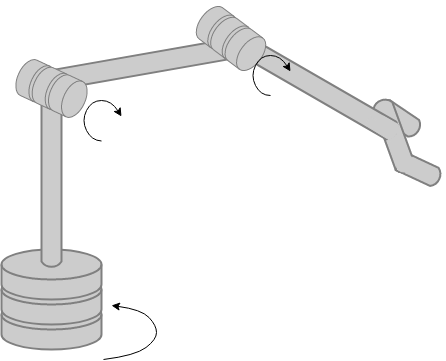
\includegraphics[width = 0.5\columnwidth]{Imagens/manipulador.png}
  \fonte{Do autor}
  \label{fig:manipuladorRRR} 
\end{figure}

\section{Sistemas de Controle}
\markright{\thesection ~~~ Sistemas de Controle}
%\label{manipRob}

Segundo \citeonline{Phillips}, um controlador é necessário em uma planta 
para processar um sinal de erro de forma a atender certas especificações pré-definidas. 
Esse sinal de erro é dado pela diferença entre a resposta do sistema, 
determinada por um sensor, e a trajetória desejada. Dentre as especificações mais 
comuns em controle de sistemas dinâmicos lineares estão: rejeição do 
distúrbio, erro em estado estacionário e a resposta transiente \cite{Ogata}.

As variedades de controle se dão conforme os tipos de sinais existentes. Sinais 
analógicos são aqueles que apresentam valor em qualquer instante de tempo, os 
sinais discretos apresentam valores em instantes múltiplos do tempo de amostragem, e 
por fim, os sinais digitais são aqueles amostrados no tempo tendo sua 
amplitude representada por um número limitado de \textit{bits}, ou seja, a amplitude 
sofre o efeito da quantização \cite{Castrucci}. Geralmente, no projeto de controladores
digitais, primeiro é realizado o projeto do controlador analógico, o qual é convertido, 
então, em digital para execução computacional. Por outro lado, existem também 
metodologias para a síntese direta de controladores digitais, as quais podem fornecer 
melhores resultados quando comparadas ao método indireto. Todavia, essas últimas são menos utilizadas.

Nos dias atuais, o controlador mais utilizado na indústria é o controlador PID. 
Segundo \citeonline{Ogata}, mais da metade dos controladores industriais empregam
o controle PID ou variantes. O seu sucesso está ligado diretamente a sua 
concepção robusta e sua aplicabilidade geral a maioria dos sistemas. O seu nome 
advém das componentes que definem a lei de controle, dada na Equação \eqref{eq:pid}, a qual é composta
pelas ações proporcional, integradora e derivativa \cite{Castrucci}:

\begin{equation}
  \begin{gathered}
    u(t) = K_p\left(e(t)+\frac{1}{T_i}\int_{0}^{t}e(\tau)d\tau+T_d\frac{de(t)}{dt}\right)
  \end{gathered}
  \label{eq:pid}
\end{equation}
com:

\begin{itemize}
 \item \textit{u(t)}: sinal de saída do controlador, ou variável manipulada;
 \item \textit{e(t)}: sinal de entrada do controlador, ou erro entre a resposta do sistema e o sinal de referência;
 \item $K_p$, $T_i$, $T_d$: parâmetros de ajustes do PID.
\end{itemize}

No escopo desta monografia, o controle PID será utilizado em conjunto com a técnica HIL apresentada 
na próxima subseção. Apesar disso, outras técnicas de controle podem ser igualmente empregadas seguindo 
a metodologia apresentada na monografia.

\section{Técnica \textit{Hardware in the Loop (HIL)}}
\markright{\thesection ~~~ Hardware in the Loop}
%\label{hil}

A idéia básica da técnica HIL é a inclusão de 
uma parte do \textit{hardware} real no \textit{loop} de simulação durante o desenvolvimento 
do sistema \cite{Bacic}. Isto é, a técnica consiste em inserir um dispositivo físico 
na malha de controle de uma simulação. Nessa técnica, uma parte do sistema é integrada 
a uma outra parte que está sendo simulada em tempo real \cite{Abourida}.

Os primeiros usos da técnica HIL estão relacionados com 
as simulações de voo \cite{Isermann}. Utilizando essa técnica, a NASA realizou simulações de alta 
fidelidade para o desenvolvimento de tecnologias de aeronaves altamente manobráveis \cite{Evans}. 
Outras aplicações dessa técnica vieram posteriormente com os testes dinâmicos de componentes 
de veículos, como, por exemplo, suspensão e corpo do carro \cite{Isermann}.

Para \citeonline{Abourida}, a técnica \textit{Hardware-in-the-Loop} (HIL) é fundamental
para simulações em tempo real; não para simular o sistema completo em tempo real, mas sim
para conectar uma parte do sistema a um modelo digital em tempo real. Além disso, essa técnica
de simulação tem como desafio o alcance da precisão de um modelo aceitável com um tempo de simulação 
digital viável \cite{Abourida}. Isso porque alguns sistemas (aqueles altamente não-lineares)
precisam de uma frequência de amostragem muito alta para alcançarem uma precisão aceitável.

A técnica HIL será utilizada nesta monografia através do uso de um computador de placa única
de tamanho reduzido (\textit{Raspberry Pi}). A \textit{Raspberry Pi} representa o \textit{Hardware} 
do método, e ela será inserida na malha de controle após a etapa de modelagem e controle no 
ambiente simulado.

\clearpage
%\include{DescricaoProcesso/DescricaoProcesso}
\chapter{Metodologia}

Neste capítulo, serão apresentadas as técnicas utilizadas para solução do problema. O projeto 
foi realizado em um ano e sua concepção foi dividida em três frentes, nomeadamente: desenvolvimento 
da solução para o modelo da planta com controlador simulado, controle da planta simulada com o 
controlador implementado em dispositivo físico (microcontrolador) e a implementação final em dispositivo real. 
As etapas pormenorizadas do projeto são as seguintes:

\begin{enumerate}
 \item Desenvolvimento da solução para o modelo da planta com controlador simulado
  \begin{enumerate}
    \item Definição e modelagem da planta de estudo;
    \item Construção do ambiente de simulação;
    \item Validação do modelo;
    \item Implementação e validação da estratégia de controle.
  \end{enumerate}
 \item Controle da planta simulada com o controlador em dispositivo físico
  \begin{enumerate}
    \item Discretização da planta de estudo seguido da obtenção da sua equação de diferenças;
    \item Discretização do controlador seguido da obtenção da sua equação de diferenças;
    \item Configuração do ambiente de testes com a planta rodando no computador, e o 
    controlador rodando no microcontrolador (comunicação UART).
  \end{enumerate}
  \item Implementação em dispositivo real
  \begin{enumerate}
    \item Configuração do ambiente com a planta real e o microcontrolador (comunicação UART);
    \item Implementação da estratégia de controle no microcontrolador;
    \item Testes de validação da estratégia de controle na planta física.
  \end{enumerate}
\end{enumerate}

\section{Desenvolvimento da solução para o modelo da planta}
\markright{\thesection ~~~ Metodologia}
\label{metodo}

A modelagem dos manipuladores robóticos visa descrever como os elos e juntas estão 
configurados fisicamente para tornar possível a configuração de sua orientação e sua posição 
\cite{paul1981robot}. Com isso, ao passar uma trajetória de referência que a 
ferramenta de trabalho deve descrever, as demais juntas se reajustam de modo a garantir 
que a ferramenta sempre esteja corretamente posicionada. A estratégia de controle deve, 
então, estar adequadamente sintonizada para garantir o seguimento acurado da trajetória.

No presente trabalho são realizadas duas modelagens para o manipulador: a modelagem 
cinemática e a modelagem dinâmica. A modelagem cinemática visa descrever a amplitude 
de movimento das juntas robóticas, ao passo que a modelagem dinâmica busca considerar 
as forças e torques que produzem o movimento, descrevendo, explicitamente, a relação 
entre força e movimento \cite{Spong}.

A principal ferramenta utilizada para se obter o modelo cinemático direto de um 
manipulador robótico é a convenção de \textit{Denavit-Hartenberg} (DH) \cite{paul1981robot}
. A modelagem dinâmica, por sua vez, pode ser realizada por meio das equações de 
textit{Euler-Lagrange}, que correspondem a um método baseado na energia do sistema 
\cite{Park}.

\subsection{Convenção de \textit{Denavit-Hartenberg}}
\markright{\thesubsection ~~~ Convenção de \textit{Denavit-Hartenberg}}
\label{DH}

Considera-se que o manipulador a ser modelado é de cadeia aberta, ou seja, um manipulador 
que o número de graus de liberdade seja igual ao número de articulações ativas.
Além disso, ele deve ser constituído por $n+1$ elos conectados por $n$ juntas, onde 
o elo $0$ é convencionalmente fixado ao solo. Assim sendo, segundo \citeonline{siciliano}, 
a equação cinemática direta para o manipulador pode ser calculada a partir de:

\begin{equation}
  \begin{gathered}
    T^0_n = A^0_1(q_1)A^1_2(q_2)\cdots A^{n-1}_n(q_n)
  \end{gathered}
  \label{eq:cinematicaDireta}
\end{equation}

A relação \eqref{eq:cinematicaDireta} se refere à transformação de coordenadas descrevendo 
a posição e a orientação do eixo $n$ em relação à base (eixo $0$) \cite{siciliano}. Segundo
\citeonline{Spong}, na convenção DH, cada transformação homogênea $A_i$ representada em
\eqref{eq:cinematicaDireta} equivale ao produto de quatro transformações básicas, apresentado a seguir:

\begin{equation*}
  \begin{gathered}
    A_i = Rot_{z,\theta_i}Trans_{z,\theta_i}Trans_{x,\alpha_i}Rot_{x,\alpha_i} \\[0.5cm]
    =\begin{bmatrix}
     \cos(\theta_i) & -\sin(\theta_i) & 0 & 0 \\
     \sin(\theta_i) & \cos(\theta_i) & 0 & 0 \\
     0 & 0 & 1 & 0 \\
     0 & 0 & 0 & 1 \\
    \end{bmatrix}
    \begin{bmatrix}
     1 & 0 & 0 & 0 \\
     0 & 1 & 0 & 0 \\
     0 & 0 & 1 & d_i \\
     0 & 0 & 0 & 1 \\
    \end{bmatrix} \\
    \times \begin{bmatrix}
     1 & 0 & 0 & a_i \\
     0 & 1 & 0 & 0 \\
     0 & 0 & 1 & 0 \\
     0 & 0 & 0 & 1 \\
    \end{bmatrix}
    \begin{bmatrix}
     1 & 0 & 0 & 0 \\
     0 & \cos(\alpha_i) & -\sin(\alpha_i) & 0 \\
     0 & \sin(\alpha_i) & \cos(\alpha_i) & d_i \\
     0 & 0 & 0 & 1 \\
    \end{bmatrix} \\
  \end{gathered}
\end{equation*}
\begin{equation}
  \begin{gathered}
    =
    \begin{bmatrix}
     \cos(\theta_i) & -\sin(\theta_i)\cos(\alpha_i) & \sin(\theta_i)\sin(\alpha_i) & a_i\cos(\theta_i) \\
     \sin(\theta_i) & \cos(\theta_i)\cos(\alpha_i) & -\cos(\theta_i)\sin(\alpha_i) & a_i\sin(\theta_i) \\
     0 & \sin(\alpha_i) & \cos(\alpha_i) & d_i \\
     0 & 0 & 0 & 1 \\
    \end{bmatrix}
  \end{gathered}
  \label{eq:matTransHomog}
\end{equation}

A matriz final encontrada em \eqref{eq:matTransHomog} é chamada de Matriz de
Trasformação Homogênea. Os quatro parâmetros da relação \eqref{eq:matTransHomog} 
representam: tamanho do elo ($a_i$), deslocamento do elo ($d_i$), 
giro do elo ($\alpha_i$), ângulo da junta ($\theta_i$). De acordo com 
\citeonline{paul1981robot}, os parâmetros são obtidos através do procedimento a seguir:

\begin{itemize}
  \item Rotacionar $x_i$ em torno do eixo $z_{i}$ um ângulo $\theta_i$;
  \item Transladar ao longo do eixo $z_{i}$ uma distância $d_i$;
  \item Transladar ao longo de $x_{i+1}$ uma distância $a_i$; 
  \item Rotacionar $z_i$ em torno de $x_{i+1}$ o ângulo de torção $\alpha_i$
\end{itemize}

Assim sendo, a modelagem cinemática é obtida através da multiplicação de diversas
matrizes de transformação homogêneas individuais, conforme
\eqref{eq:cinematicaDireta}. Com isso, para um manipulador com três graus de 
liberdade, a transformação de coordenadas do elemento terminal em relação a base é
dada por $T^0_3=A_1A_2A_3$ .

\subsubsection{Cinemática Diferencial e o Jacobiano}

A cinemática diferencial é responsável por fornecer a relação entre as velocidades das juntas
e a correspondente velocidade final linear e angular da ferramenta de trabalho \cite{siciliano}. Essa 
relação é descrita por uma matriz denominada jacobiana geométrica, que depende da configuração do manipulador. 
O Jacobiano Analítico, por outro lado, é expresso por meio da diferenciação da função cinemática direta com 
relação às variáveis das juntas. A obtenção da matriz Jacobiana é fundamental para determinar as equações 
de movimento do manipulador robótico.

Segundo \citeonline{Spong}, considerando um manipulador com \textit{n} graus de liberdade, a equação da cinemática direta 
pode ser escrita na forma:

\begin{equation}
  \begin{gathered}
    T^{0}_n(q) = \begin{bmatrix}
     R^{0}_n(q) & o^{0}_n(q)\\
     0 & 1\\
    \end{bmatrix}
  \end{gathered}
  \label{eq:cinematicaDireta_2}
\end{equation}

A equação \eqref{eq:cinematicaDireta_2} é a mesma que \eqref{eq:cinematicaDireta}, onde $q = [q_1,...,q_n]^T$ é o vetor das 
variáveis das juntas, $R^{0}_n(q)$ a matriz de rotação, $o^{0}_n(q)$ o vetor de translação, $0$ a perspectiva e $1$ o 
fator de escala. As relações da velocidade linear $v^0_n$ e a velocidade angular $\omega^0_n$ em função das velocidades 
das juntas é linear \cite{siciliano} e pode ser expressa por:

\begin{equation}
  \begin{gathered}
    v^0_n = J_v \dot{q}
  \end{gathered}
  \label{eq:jacob_velLinar}
\end{equation}

\begin{equation}
  \begin{gathered}
    \omega^0_n = J_\omega \dot{q}
  \end{gathered}
  \label{eq:jacob_velAngular}
\end{equation}
onde $J_v$ e $J_\omega$ são matrizes $3 \times n$. É possível ainda, reescrever \eqref{eq:jacob_velLinar} e
\eqref{eq:jacob_velAngular} da seguinte forma:
\begin{equation}
  \begin{gathered}
    \zeta = J\dot{q}
  \end{gathered}
  \label{eq:jacob_ambos}
\end{equation}

\begin{equation}
  \begin{gathered}
    \zeta = \begin{bmatrix}
     v^0_n\\
     \omega^0_n\\
    \end{bmatrix}
    \quad \textrm{e} \quad 
    J = \begin{bmatrix}
     J_v\\
     J_\omega\\
    \end{bmatrix}
  \end{gathered}
\end{equation}

O vetor $\zeta$ também pode ser chamado de velocidade do corpo \cite{Spong} e é importante notar que
ele não é a derivada de uma variável de posição. A matriz $J$ é chamado de \textbf{Jacobiano} e trata-se
de uma matriz $6 \times n$ .

Combinando as partes angular e linear, segundo \citeonline{siciliano}, a metade de cima da matriz do Jacobiano é
dada por:

\begin{equation}
  \begin{gathered}
    J_{v_i} = 
      \left\{
	\begin{array}{cl}
	  z_{i-1} \times (o_n - o_{i-1}) & \text{para a $i$-ésima junta revoluta}\\
	  z_{i-1} 			 & \text{para a $i$-ésima junta prismática}
	\end{array}
      \right.
  \end{gathered}
\end{equation}

A segunda metade, ou a metade baixo da matriz do Jacobiano é dada por:

\begin{equation}
  \begin{gathered}
    J_{\omega_i} = 
      \left\{
	\begin{array}{cl}
	  z_{i-1} & \text{para a $i$-ésima junta revoluta}\\
	  0 	  & \text{para a $i$-ésima junta prismática}
	\end{array}
      \right.
  \end{gathered}
\end{equation}

Juntando ambas as metades da matriz do Jacobiano obtém-se para a junta revoluta a equação \eqref{eq:revolJacobiano}
e para a junta prismática \eqref{eq:prismaticJacobiano}:

\begin{equation}
  \begin{gathered}
    J_i = \begin{bmatrix}
     z_{i-1} \times (o_n - o_{i-1})\\
     z_{i-1}\\
    \end{bmatrix}
  \end{gathered}
  \label{eq:revolJacobiano}
\end{equation}

\begin{equation}
  \begin{gathered}
    J_i = \begin{bmatrix}
     z_{i-1}\\
     0\\
    \end{bmatrix}
  \end{gathered}
  \label{eq:prismaticJacobiano}
\end{equation}

Assim sendo, as únicas ferramentas necessárias para calcular o Jacobiano são os 
vetores unitários $z_i$ e as coordenadas das origens $o_1, ..., o_n$. As coordenadas
para $z_i$ são dadas pelos três primeiros elementos da terceira coluna de $T^0_i$, 
enquanto as coordenadas de $o_n$ são dadas pelos três primeiros elementos da quarta
coluna de $T^0_i$ . Dessa forma, apenas a terceira e a quarta colunas da matriz de 
homogeneidade $T$ são necessárias para obter o Jacobiano. \cite{Spong}

\subsection{Equações de \textit{Euler-Lagrange}}
\markright{\thesubsection ~~~ Equações de \textit{Euler-Lagrange}}
\label{EL}

Com o conjunto de coordenadas generalizadas independentes $q_j$, $j = 1, \dotsc, n$, onde $n$ 
representa os graus de liberdade do manipulador, o Lagrangiano do sistema 
é definido pela relação \eqref{eq:lagrangiano} \cite{Spong}, onde $K$ representa 
a energia cinética e $P$ a energia potencial do sistema:

\begin{equation}
  \begin{gathered}
    L = K - P
  \end{gathered}
  \label{eq:lagrangiano}
\end{equation}

Segundo \citeonline{Spong}, em geral, as equações de \textit{Euler-Lagrange}
aplicadas a um sistema de $n$ coordenadas podem ser representadas na forma da
Equação \eqref{eq:EL}, onde a força generalizada $\tau_i$ representa as forças 
externas e torques não deriváveis de uma função potencial:

\begin{equation}
  \begin{gathered}
    \frac{d}{dt}\frac{\partial L}{\partial \dot q_i}-\frac{\partial L}{\partial q_i} = \tau_i
  \end{gathered}
  \label{eq:EL}
\end{equation}

Conforme apresentado, as equações de \textit{Euler-Lagrange} podem ser 
usadas para derivar as equações dinâmicas de maneira direta. É possível computar 
esses termos para um manipulador robótico de $n$ elos por meio das fórmulas da 
energia cinética e da energia potencial usando as variáveis de articulação obtidas a partir da modelagem 
de \textit{Denavit-Hartenberg} como coordenadas generalizadas \cite{Spong}.

\subsubsection{Energia cinética para um manipulador de $n$ elos}

Segundo \citeonline{Spong} a energia cinética é dada pela soma de dois 
termos: a energia de translação, obtida concentrando toda a massa do objeto no 
centro de massa, e a energia cinética rotacional em torno do centro de massa. 
Assim, a energia cinética do manipulador é dada por:

\begin{equation}
  \begin{gathered}
    K=\frac{1}{2}mv^Tv+\frac{1}{2}\omega^T\Gamma \omega
  \end{gathered}
  \label{eq:energiaCinetica}
\end{equation}
onde $m$ é a massa do objeto, $v$ e $\omega$ são os vetores de velocidade 
linear e angular, respectivamente, e $\Gamma$ é uma matriz simétrica $3 \times 3$ 
chamada Tensor de Inércia. O Tensor de Inércia é relacionado ao quadro de 
referência inercial do manipulador. Dessa forma, é possível 
relacionar o tensor de inércia com a matriz de rotação através de uma 
transformação de similaridade:

\begin{equation}
  \begin{gathered}
    \Gamma = RIR^T
  \end{gathered}
  \label{eq:ts}
\end{equation}
onde $R$ é a matriz de rotação $R^{0}_n(q)$ obtida em \eqref{eq:jacob_velLinar}, e 
$I$ é uma matriz que não depende do movimento do objeto. 
Cada elemento dessa matriz é calculado através de integrais sobre as
regiões do espaço ocupados por todas as partes do corpo rígido:

\begin{equation}
  \begin{gathered}
    I = \begin{bmatrix}
     I_{xx} & I_{xy} & I_{xz}\\
     I_{yx} & I_{yy} & I_{yz}\\
     I_{zx} & I_{zy} & I_{zz}\\
    \end{bmatrix}
  \end{gathered}
\end{equation}

\begin{equation}
  \begin{gathered}
    I_{xx} = \iiint(y^2+z^2)\rho(x,y,z)dxdydz\\
    I_{yy} = \iiint(x^2+z^2)\rho(x,y,z)dxdydz\\
    I_{zz} = \iiint(x^2+y^2)\rho(x,y,z)dxdydz\\
    I_{xy} = I_{yx} = - \iiint xy\rho(x,y,z)dxdydz\\
    I_{xz} = I_{zx} = - \iiint xz\rho(x,y,z)dxdydz\\
    I_{yz} = I_{zy} = - \iiint yz\rho(x,y,z)dxdydz\\
  \end{gathered}
\end{equation}

Através do Tensor de Inércia, do jacobiano, da matriz de rotação e da massa de
cada parte do braço obtém-se a energia cinética do manipulador:

\begin{equation}
  \begin{gathered}
    K=\frac{1}{2}\dot q^T D(q)\dot q
  \end{gathered}
  \label{eq:ecMat}
\end{equation}
sendo:
\begin{equation}
  \begin{gathered}
    D(q)= \sum^n_{i=1}[m_iJ_{vi}(q)^TJ_{vi}(q)+J_{\omega i}(q)^TR_i(q)I_i(q)R_i(q)^TJ_{\omega i}(q)]
  \end{gathered}
  \label{eq:dq}
\end{equation}

\subsubsection{Energia potencial para um manipulador de $n$ elos}

A energia potencial do manipulador de $n$ elos é dada pela soma da energia
potencial individual de cada parte envolvida. A única fonte de energia potencial
do manipulador é a gravidade, assumindo que a massa total de cada elemento 
do manipulador está concentrada no seu centro de massa.

Segundo \citeonline{Spong}, a energia potencial é uma função apenas das 
coordenadas generalizadas e não de suas derivadas, assim, a energia 
potencial depende da configuração do robô e independe da velocidade:

\begin{equation}
  \begin{gathered}
    P = \sum^n_{i=1}P_i = \sum^n_{i=1}g^Tr_{ci}m_i
  \end{gathered}
  \label{eq:enePotencial}
\end{equation}
onde $g$ é o vetor que dá a direção da gravidade no referencial inercial, e 
$r_{ci}$ fornece as coordenadas do centro de massa do elo $i$. Sendo assim,
a matriz da energia potencial é dada por:

\begin{equation}
  \begin{gathered}
    g(q)=\phi_k=\frac{\partial P}{\partial q_k}
  \end{gathered}
  \label{eq:enePotencialMat}
\end{equation}

\subsubsection{Equações de movimento}

Aplicando o que foi exposto anteriormente, as equações de \textit{Euler-Lagrange} 
\eqref{eq:EL} podem ser expressas segundo:

\begin{equation}
  \begin{gathered}
    \sum_i d_{kj}(q)\ddot q_j + \sum_{i,j}c_{ijk}(q)\dot q_i\dot q_j + \phi_k = \tau_k \quad, \quad k=1,\dots,n
  \end{gathered}
  \label{eq:EL_Final}
\end{equation}
ou na forma matricial:
\begin{equation}
  \begin{gathered}
    D(q)\ddot q + C(q,\dot q)\dot q + g(q) = \tau
  \end{gathered}
  \label{eq:EL_FinalMat}
\end{equation}
onde $D(q)$ e $g(q)$ representam as matrizes da energia cinética e potencial, 
respectivamente, e $C(q,\dot q)$ representa uma matriz construída com os chamados
Símbolos de Christoffel, definidos matematicamente por \citeonline{Spong} através
da equação:

\begin{equation}
  \begin{gathered}
    c_{ijk} = \frac{1}{2} \left\{ \frac{\partial d_{kj}}{\partial q_i}+\frac{\partial d_{ki}}{\partial q_j}-\frac{\partial d_{ij}}{\partial q_k} \right\}
  \end{gathered}
  \label{eq:christoffel}
\end{equation}

Como o manipulador RRR possui três juntas revolutas, e cada junta revoluta é descrita por uma matriz 
$3 \times 3$, serão necessários 27 Símbolos de Christoffel diferentes.

\section{Ensaio em malha aberta para a obtenção do modelo da planta}

O modelo matemático de um sistema é definido como um conjunto de equações que representa a sua dinâmica \cite{Ogata}. 
Esses modelos são sempre idealizações do comportamento
real e são válidos para excitações dentro de certos limites de amplitude e frequência \cite{Castrucci}.

Uma das formas de se obter o modelo de um determinado sistema $G(s)$, dentro de certos limites de amplitude e frequência,
é através dos seus dados de entrada $U(s)$ e saída $Y(s)$, vide \autoref{fig:diagEnsaioMA}. Ao aplicar na entrada uma 
referência conveniente (degrau, impulso, senoide), ignorando os fenômenos internos, obtém-se uma determinada saída que ao 
ser avaliada ao longo do tempo, ficam aparentes os parâmetros das equações diferenciais procuradas \cite{Castrucci}.

\begin{figure}[ht]
  \centering
  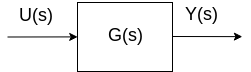
\includegraphics[width = 0.4\columnwidth]{Imagens/diagEnsaioMA.png}
  \caption{Diagrama do ensaio em malha aberta}
  \fonte{Do autor}
  \label{fig:diagEnsaioMA} 
\end{figure}

A resposta temporal de um sistema de controle é composto da resposta transitória, aquela que compreende o tempo entre o 
estado inicial e o final, e a resposta estacionária que corresponde ao comportamento do sinal de saída quando $t$
tende ao infinito \cite{Ogata}. Dependendo do comportamento das respostas do sistema, ele pode ser classificado
como de primeira ordem \eqref{eq:sistemaPrimeiraOrdem}, de segunda ordem \eqref{eq:sistemaSegundaOrdem} ou como sistema 
de ordem superior.

\begin{equation}
  \begin{gathered}
    \frac{Y(s)}{U(s)} = \frac{1}{\tau s + 1}
  \end{gathered}
  \label{eq:sistemaPrimeiraOrdem}
\end{equation}

\begin{equation}
  \begin{gathered}
    \frac{Y(s)}{U(s)} = \frac{\omega_n^2}{s^2 + 2\xi \omega_n s + \omega_n^2}
  \end{gathered}
  \label{eq:sistemaSegundaOrdem}
\end{equation}
onde:

\begin{itemize}
 \item $\tau$: constante de tempo do sistema ($\tau > 0$);
 \item $\omega_n$: frequência natural não amortecida ($\omega_n > 0$);
 \item $\xi$: coeficiente de amortecimento.
\end{itemize}

A constante de tempo do sistema de primeira ordem é definida como o instante em que a resposta 
do sistema atingiu 63,2\% de sua variação final \cite{Castrucci}. Por outro lado, para os sistemas de
segunda ordem, o que define o $\xi$ é o sobressinal máximo do sistema, e o $\omega_n$ pode ser definido
pelas constantes de tempo do sistema de segunda ordem, como por exemplo o tempo de 
acomodação. O tempo de acomodação para uma faixa de $\pm$ 2\% em torno do valor final é dado 
por \eqref{eq:tempoAcomodacao}:

\begin{equation}
  \begin{gathered}
    t_s \cong \frac{4}{\xi \omega_n}
  \end{gathered}
  \label{eq:tempoAcomodacao}
\end{equation}

\section{Projeto de sistemas de controle pelo método do lugar das raízes}

O lugar das raízes é um método simples que possibilita a representação gráfica das raízes da equação
característica para todos os valores do ganho, ou qualquer outro parâmetro da função de transferência
de malha aberta \cite{Ogata}. O projeto de controle pelo método do lugar das raízes é realizado através 
da adição de zeros e polos à função de transferência de malha aberta do sistema, forçando o lugar das raízes a passar 
pelos polos de malha fechada desejados.

No presente projeto, foram levantados três modelos para planta, um para cada uma das juntas (base, ombro, cotovelo).
Para cada uma delas foi projetado um controlador independe (conhecido na literatura como controle de juntas independes). Os projetos 
foram realizado através do método do lugar das raízes, com o auxílio da ferramenta \textit{sisotool} do \textit{Matlab}.

\section{Configuração do ambiente de simulação}

A partir dos modelos cinemáticos e dinâmicos obtidos, um ambiente de simulação é 
concebido na plataforma \textit{Matlab} (\autoref{fig:plantaSimulada}). Por meio desse 
ambiente, diferentes técnicas de controle podem ser sintetizadas e validadas para o manipulador estudado. 
Posteriormente, é feita a implementação da estratégia de controle sintetizada em dispositivo físico (microcontrolador),
sendo que a validação é realizada no ambiente de simulação 
desenvolvido por meio da técnica HIL, vide 
\autoref{fig:solucaoModelo}. Finalmente, a última etapa corresponde à implementação das 
estratégias de controle no manipulador robótico estudado (planta física). Como ilustrado 
na \autoref{fig:solucaoPlanta}, nessa etapa o microntrolador é conectado ao manipulador de 
forma a controlá-lo, fazendo-o seguir uma trajetória pré-especificada. Assim, verifica-se 
se, de fato, a resposta do sistema físico em malha fechada corresponde à resposta obtida 
por meio de simulação utilizando a técnica HIL.

\begin{figure}[h!]
  
  \centering
  \begin{subfigure}{.5\textwidth}
    \centering
    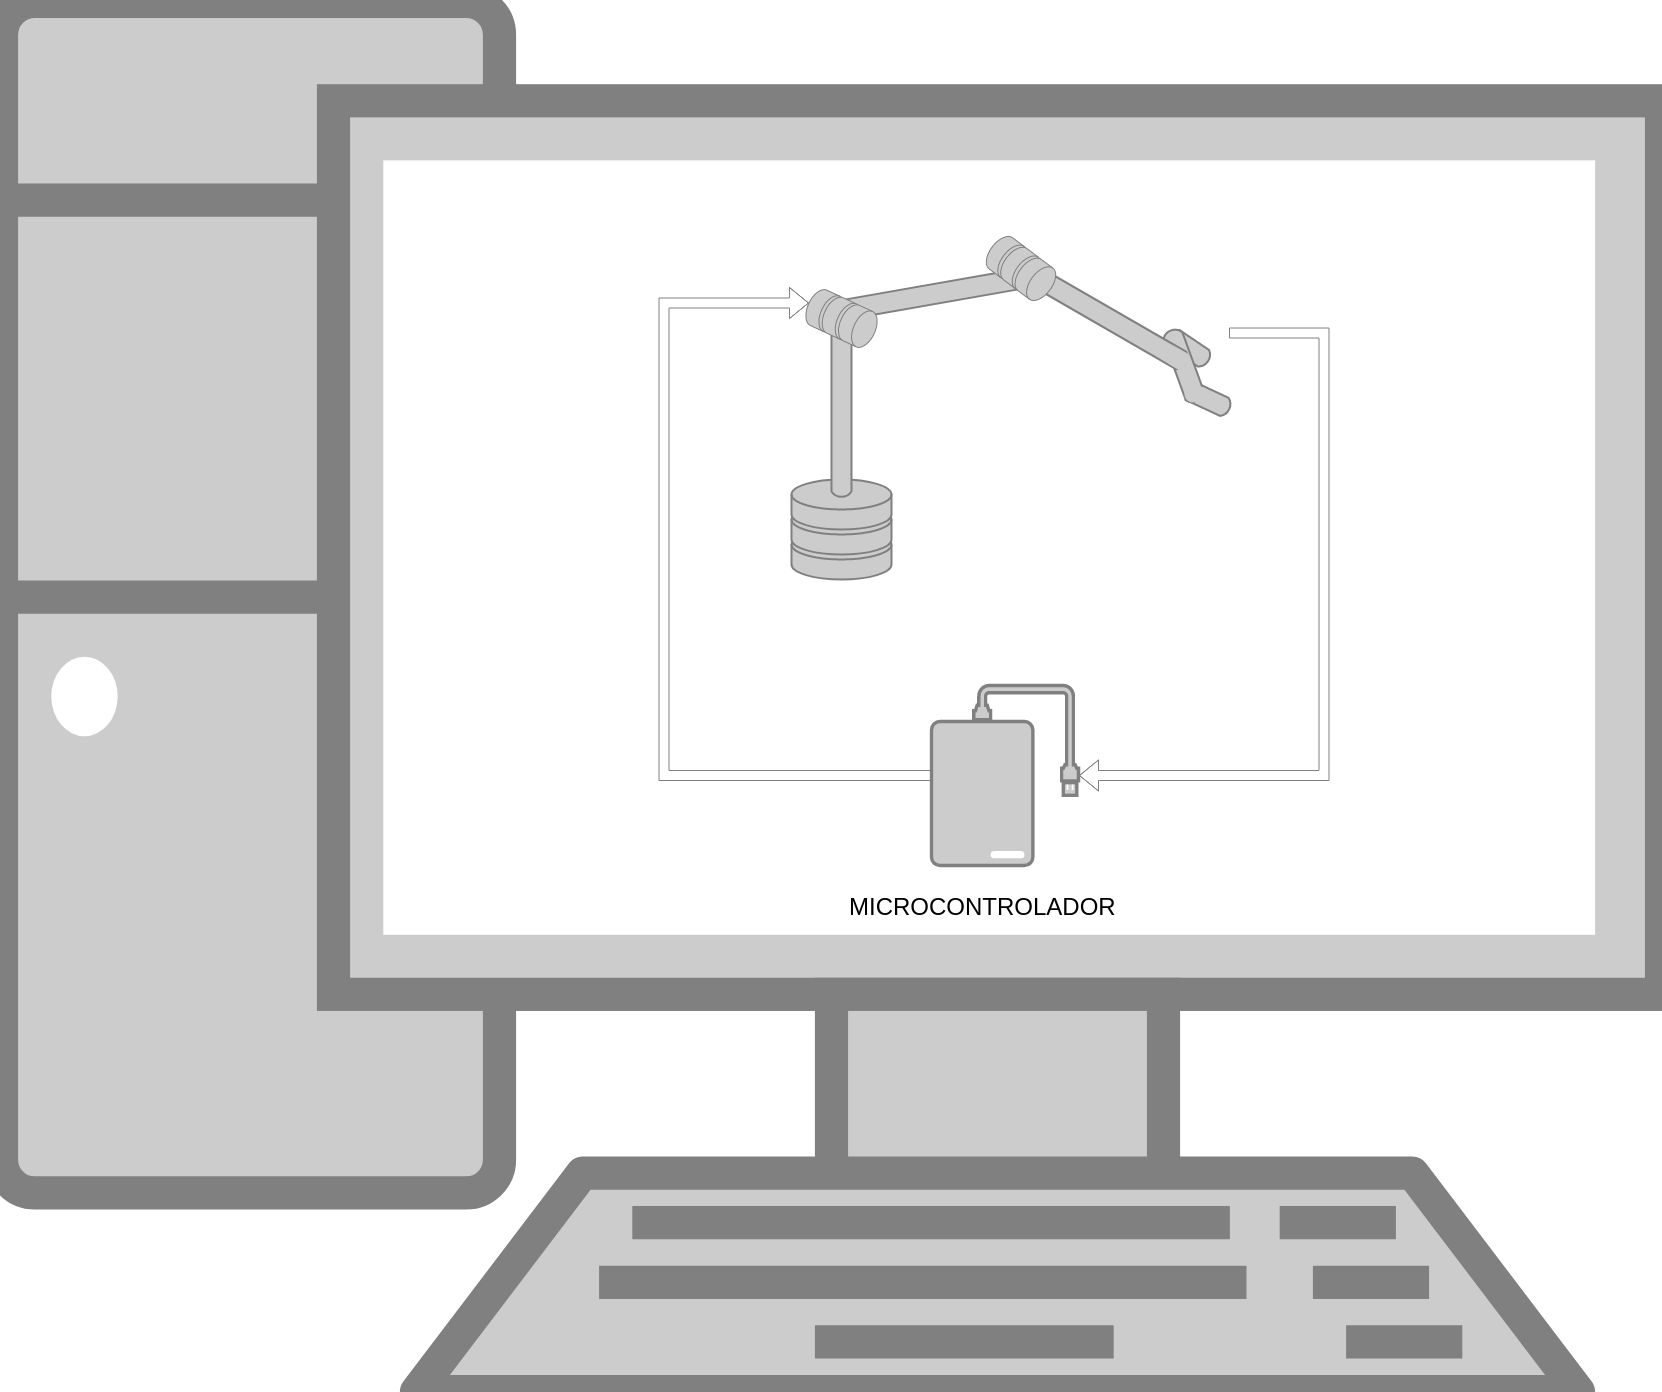
\includegraphics[width = 0.6\columnwidth]{Imagens/plantaSimulada.png}
    \caption{Planta e controlador simulados}
    \fonte{Do autor}
    \label{fig:plantaSimulada}
  \end{subfigure}%
  \begin{subfigure}{.5\textwidth}
    \centering
    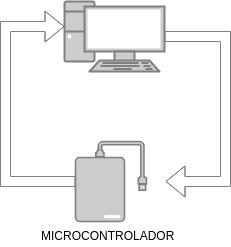
\includegraphics[width = 0.5\columnwidth]{Imagens/solucaoModelo.png}
    \caption{Solução para o modelo simulado da planta}
    \fonte{Do autor}
    \label{fig:solucaoModelo}
  \end{subfigure}%
  \\[5ex]
  \begin{subfigure}{\textwidth}
    \centering
    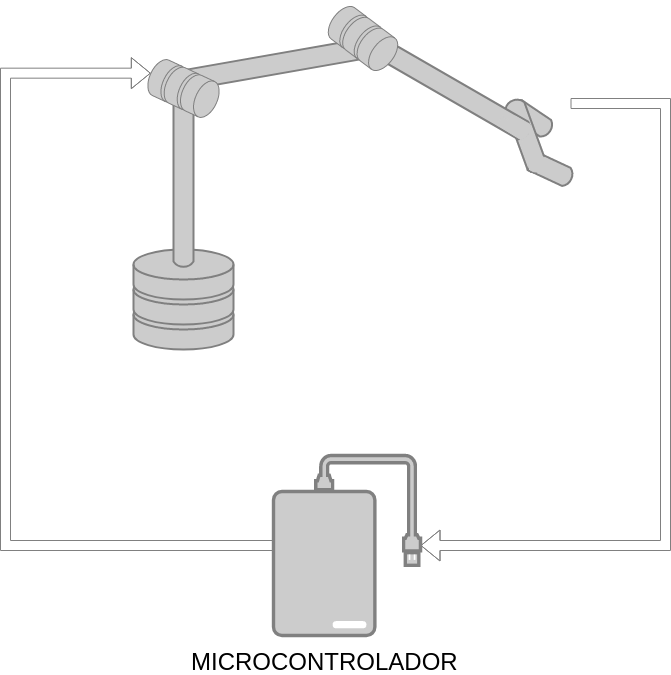
\includegraphics[width = 0.4\columnwidth]{Imagens/solucaoPlanta.png}
    \caption{Solução para a planta física}
    \fonte{Do autor}
    \label{fig:solucaoPlanta}
  \end{subfigure}%
  \caption{Diagramas das etapas da técnica \textit{Hardware-in-the-loop}}
  
  \label{fig:simulacoes} 

\end{figure}

\section{Resumo do Capítulo}
\markright{\thesection ~~~ Metodologia}
\label{metodo1b}

Este capítulo apresentou de forma sucinta a metodologia de projeto seguida para 
alcançar os objetivos propostos neste trabalho. No próximo capítulo são realizadas 
as modelagens cinemática e dinâmica do manipulador, a partir das quais o ambiente de 
simulação foi construído.


\clearpage
\chapter{Resultados}
%\markboth{\thechapter ~~~ Resultados}{}
%\label{result}

Neste capítulo, os resultados para o projeto descritos no capítulo anterior serão apresentados. A obtenção do modelo da 
planta foi dada de duas formas diferentes: por meio da convenção de \textit{Denavit-Hartenberg} e equações de 
\textit{Euler-Lagrange} e por meio do ensaio em malha aberta. Para o primeiro método, foram feitas algumas considerações,
dadas a seguir:
\begin{enumerate}
 \item O elo do cotovelo e o elo do ombro são barras de comprimento $L$ e massa $m$, e possuem o eixo de rotação no fim
 da barra;
 \item O elo da base é um cilindro sólido de raio $r$, altura $h$ e massa $m$;
 \item A distribuição de massa de cada elo com a sua junta respectiva é simétrica em relação à estrutura do corpo, ou seja,
 a massa está uniformemente distribuída ao longo do corpo.
\end{enumerate}

O código em MATLAB referente ao modelo obtido por meio da convenção de \textit{Denavit-Hartenberg} e equações de
\textit{Euler-Lagrange} é apresentado no \refanexo{anexo:denHatEulerLagr}. A \autoref{fig:dh_simulation} mostra 
o modelo encontrado por meio da matriz de homogeneidade resultante da convenção DH. Nota-se a coerência deste 
modelo com o manipulador real por respeitar a proporção e distribuição dos elos e juntas.

\begin{figure}[ht]
  \centering
  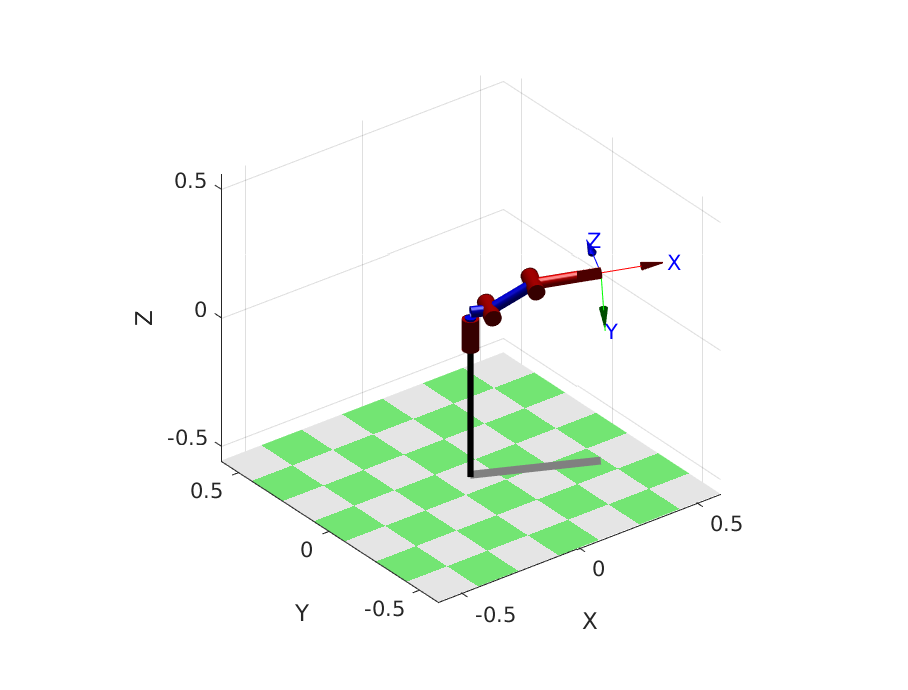
\includegraphics[width = 0.7\columnwidth]{Imagens/dh_simulation}
  \caption{Gráfico da representação \textit{Denavit-Hartenberg} obtida}
  \fonte{Do autor}
  \label{fig:dh_simulation}
\end{figure}

As considerações citadas no início deste capítulo, em conjunto com a complexidade na obtenção dos Símbolos de \textit{Christoffel}
tornaram a modelagem EL inviável. A solução mais coerente encontrada foi a execução do ensaio em malha aberta para a obtenção do modelo 
de cada junta do manipulador, seguido do controle de junta independente

Os modelos da planta usados para projetar os controladores foram obtidos através de ensaios em malha aberta (MA) e seguem 
na próxima seção. Três modelos foram levantados: um para a base, um para o ombro e outro para o cotovelo, e para 
cada um deles foi projetado um controlador. Esse processo é conhecido na literatura como controle de juntas independentes.

\section{Ensaio em malha aberta}
\markright{\thesection ~~~ Resultado ensaio em malha aberta}

A comunicação com os servomotores foi feita inicialmente com um computador através da porta serial com o protocolo 
UART. A linguagem usada para a execução do ensaio em malha aberta foi o \textit{Python}, e seu código completo
encontra-se disponível em \cite{lelis_model}.

Para cada uma das juntas foi feita uma montagem semelhante a apresentada na \autoref{fig:diagEnsaioMA}. Foi aplicada na entrada de
cada um dos servomotores uma referência em degrau para o ângulo $\theta$ (em graus). Inicialmente, o sistema tinha sido
configurado para um tempo de amostragem de $0,01s$. De acordo com a resposta obtida, observou-se uma superamostragem dos dados,
e, devido a isso, o tempo de amostragem foi reajustado empiricamente para $0,23s$. Os ângulos de resposta (em graus) obtidos
ao longo do tempo para cada uma das juntas são apresentados na \autoref{fig:ensaioMalhaAberta}.

\begin{figure}[h!]
  
  \centering
  \begin{subfigure}{.5\textwidth}
    \centering
    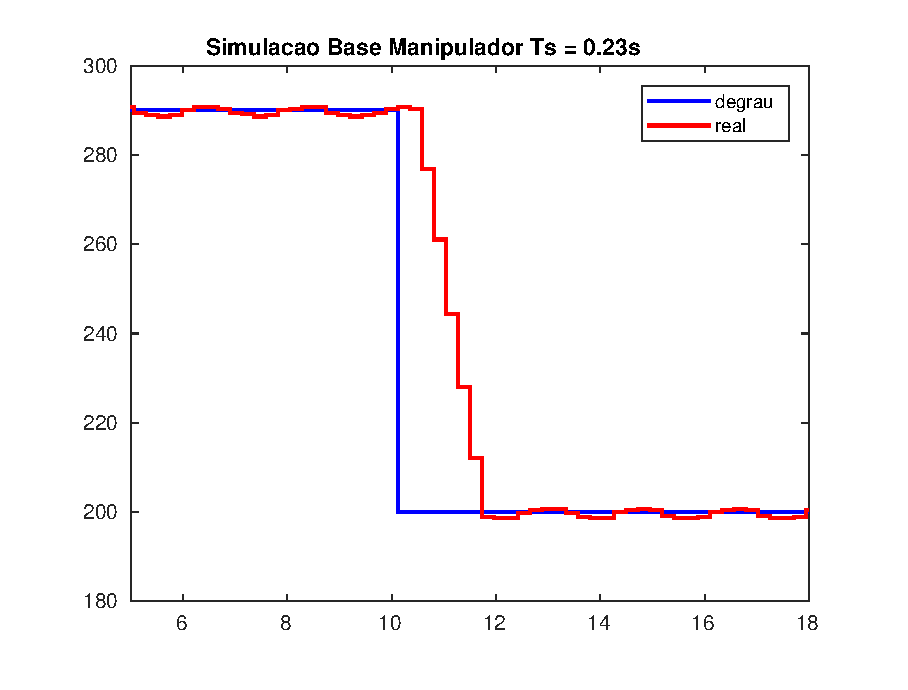
\includegraphics[width = 1.1\columnwidth]{Imagens/base_ma}
    \caption{Base}
    \fonte{Do autor}
    \label{fig:base_ma}
  \end{subfigure}%
  \begin{subfigure}{.5\textwidth}
    \centering
    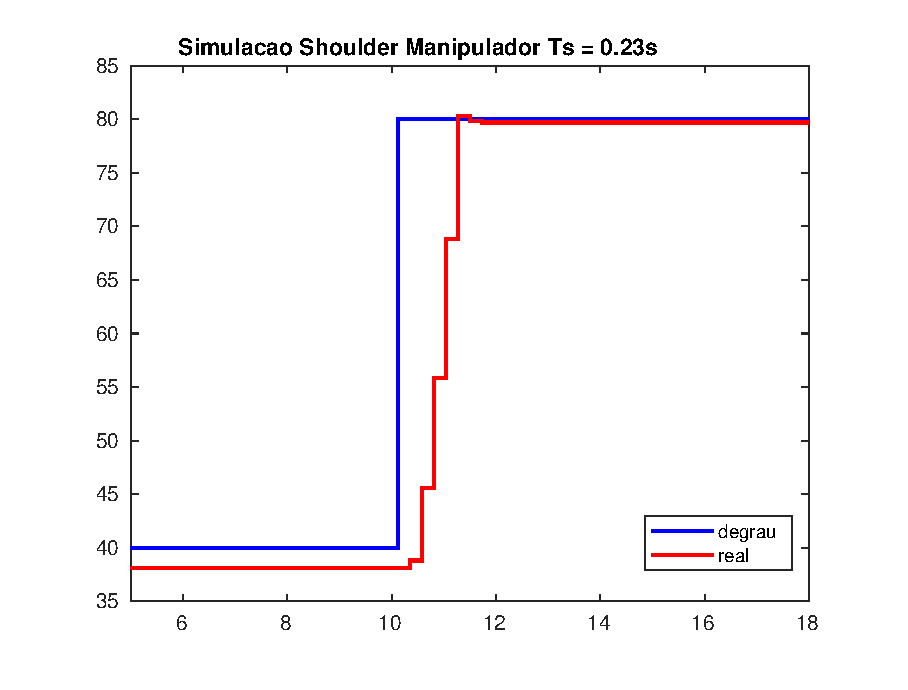
\includegraphics[width = 1.1\columnwidth]{Imagens/shoulder_ma}
    \caption{Ombro}
    \fonte{Do autor}
    \label{fig:shoulder_ma}
  \end{subfigure}%
\end{figure}

\newpage

\begin{figure}[h!]\ContinuedFloat
  \begin{subfigure}{\textwidth}
    \centering
    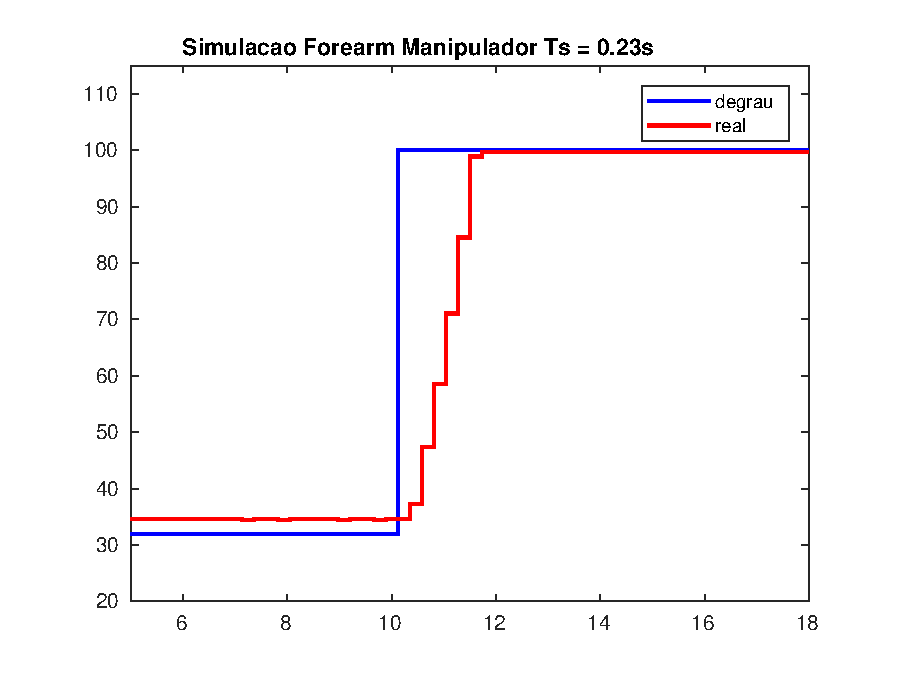
\includegraphics[width = 0.55\columnwidth]{Imagens/forearm_ma}
    \caption{Cotovelo}
    \fonte{Do autor}
    \label{fig:forearm_ma}
  \end{subfigure}%
  \caption{Gráficos da entrada e resposta para o ensaio em MA de cada uma das juntas}
  \label{fig:ensaioMalhaAberta}
\end{figure}

A princípio, observando as respostas em malha aberta das juntas, a dinâmica de cada uma poderia ser aproximada por
um modelo de primeira ordem. Entretanto, constatou-se experimentalmente que um modelo de segunda ordem, 
conforme \eqref{eq:sistemaSegundaOrdem}, era mais apropriado para descrever a dinâmica de cada junta do sistema.
Tal fato se deve, possivelmente, ao controlador interno presente nos servomotores.

Observando as Figuras \ref{fig:base_ma} e \ref{fig:forearm_ma}, observa-se um comportamento próximo do 
amortecimento crítico. Quando ocorre esse tipo de comportamento, pode-se escolher $\xi=1$ na função de 
transferência. Por outro lado, em \ref{fig:shoulder_ma}, observa-se
um pequeno sobressinal, o que resulta em um $\xi$ menor, aproximando-se para este caso: $\xi = 0,8$.

O tempo de acomodação, definido em \eqref{eq:tempoAcomodacao}, variou para todas as juntas na 
faixa $0,9s < t_s < 1,3s$. De acordo com testes qualitativos para a validação do modelo, e pelas Figuras 
\ref{fig:base_ma}, \ref{fig:shoulder_ma} e \ref{fig:forearm_ma}, foi considerado para a base, ombro e
cotovelo respectivamente: $t_s = 1,0952s$, $t_s = 0,9333s$, $t_s = 1,0952s$. Dessa forma, substituindo em 
\eqref{eq:tempoAcomodacao} as constantes encontradas por aproximação, obtém-se para as frequências naturais de
oscilação ($\omega_n$) da base, ombro e
cotovelo respectivamente: $\omega_n = 3.6522 rad/s$, $\omega_n = 5.3571 rad/s$, $\omega_n = 3.6522 rad/s$.
O valor das variáveis encontradas para cada uma das juntas segue na \autoref{tab:ctesModeloMA}

\begin{center}
    \captionof{table}{Constantes determinadas para os modelos das juntas}
    \begin{tabular}{| c | c | c | c |}\hline
      \textbf{Junta}	& $\xi$ 	& $t_s$ (s)	& $\omega_n$ (rad/s)	\\ \hline
      Base		& 1 		& 1,0952	& 3,6522		\\ \hline
      Ombro		& 0,8 		& 0,9333	& 5,3571		\\ \hline
      Cotovelo		& 1 		& 1,0952	& 3,6522		\\ \hline
    \end{tabular}
    \label{tab:ctesModeloMA}
\end{center}

\section{Fase 1 da técnica HIL - Planta e controlador simulados}
\markright{\thesection ~~~ Fase 1 da técnica HIL}

Como foi exposto na seção anterior, as constantes foram encontradas por aproximações de acordo
com o que foi observado no ensaio em malha aberta. A partir disso, as funções de transferência
para a base, ombro e cotovelo foram obtidas através da Equação \eqref{eq:sistemaSegundaOrdem} e 
seguem respectivamente em \eqref{eq:baseModel}, \eqref{eq:shoulderModel} e \eqref{eq:forearmModel}:
\begin{equation}
  \begin{gathered}
    G(s) = \frac{13,3384}{s^2 + 7,3043s + 13,3384}
  \end{gathered}
  \label{eq:baseModel}
\end{equation}

\begin{equation}
  \begin{gathered}
    G(s) = \frac{0,9965 \cdot 28,69898}{s^2 + 8,5714s + 28,69898}
  \end{gathered}
  \label{eq:shoulderModel}
\end{equation}

\begin{equation}
  \begin{gathered}
   G(s) = \frac{13,3384}{s^2 + 7,3043s + 13,3384}
  \end{gathered}
  \label{eq:forearmModel}
\end{equation}

Os mesmos degraus aplicados na planta real, foram aplicados nas funções de transferência para
validação dos modelos. Os resultados obtidos seguem na \autoref{fig:base_ma_simul}, na
\autoref{fig:shoulder_ma_simul} e na \autoref{fig:forearm_ma_simul}.

\begin{figure}[h!]
  
  \centering
  \begin{subfigure}{.5\textwidth}
    \centering
    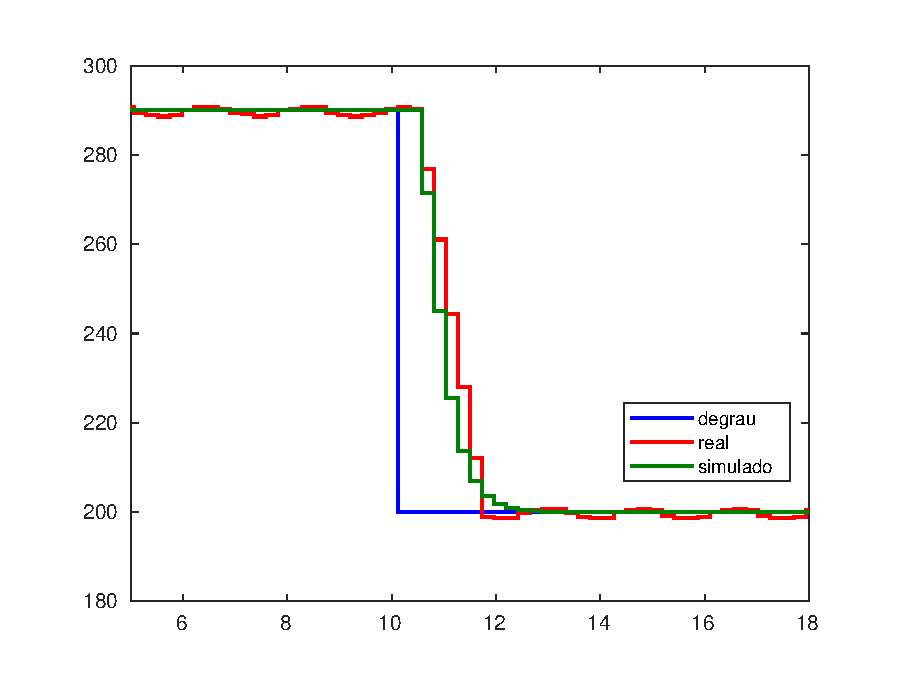
\includegraphics[width = .8\columnwidth]{Imagens/base_ma_simul}
    \caption{Base}
    \fonte{Do autor}
    \label{fig:base_ma_simul}
  \end{subfigure}%
  \begin{subfigure}{.5\textwidth}
    \centering
    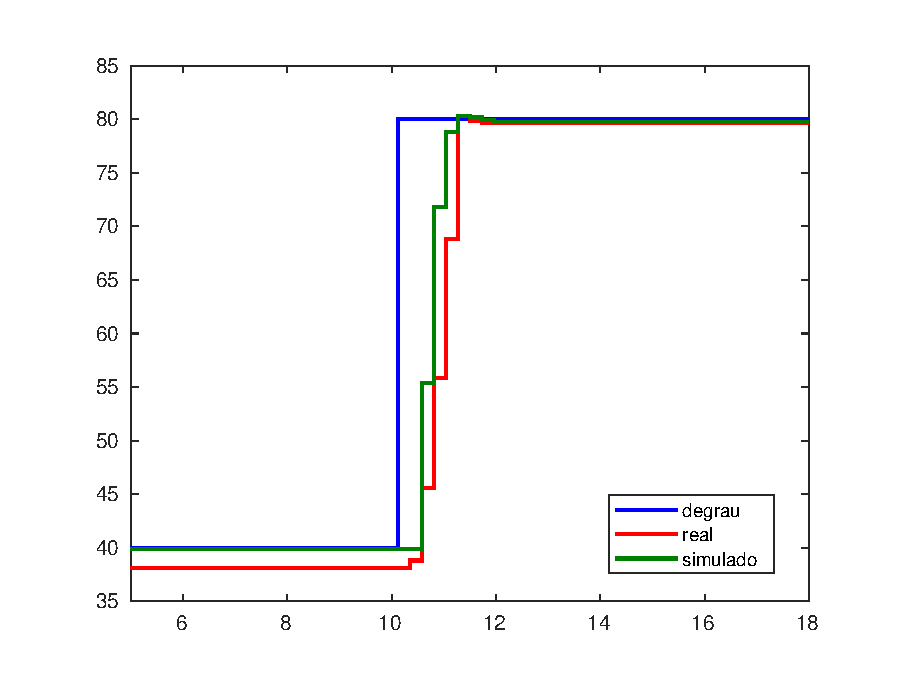
\includegraphics[width = .8\columnwidth]{Imagens/shoulder_ma_simul}
    \caption{Ombro}
    \fonte{Do autor}
    \label{fig:shoulder_ma_simul}
  \end{subfigure}%
  \\
  \begin{subfigure}{\textwidth}
    \centering
    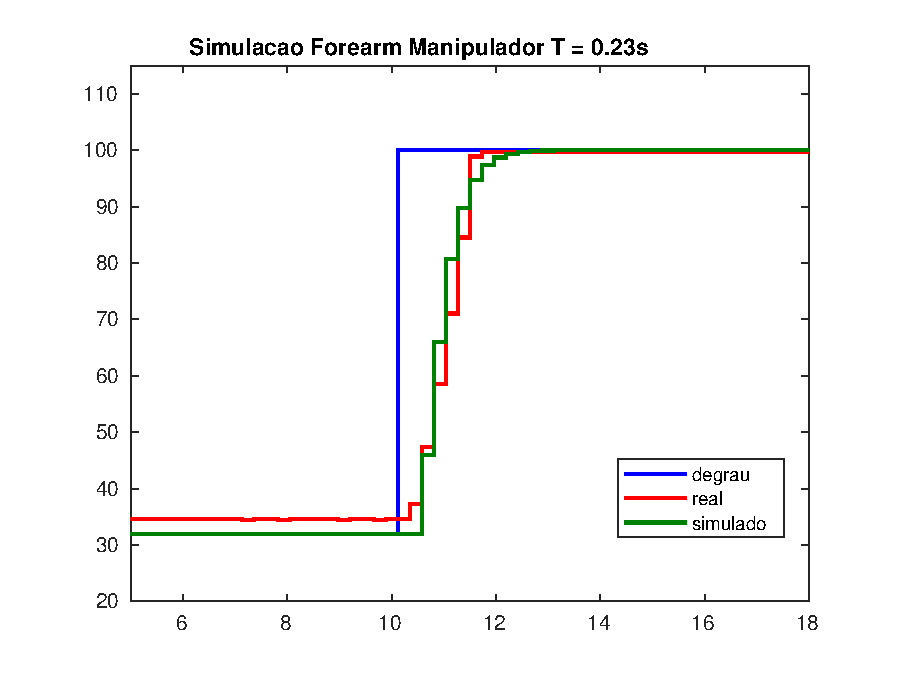
\includegraphics[width = 0.4\columnwidth]{Imagens/forearm_ma_simul}
    \caption{Cotovelo}
    \fonte{Do autor}
    \label{fig:forearm_ma_simul}
  \end{subfigure}%
  \caption{Gráficos da entrada e resposta do modelo obtido para cada uma das juntas}
  \label{fig:ensaioMalhaAbertaSimul} 

\end{figure}

Note que as curvas simuladas aproximam adequadamente as respostas de cada junta em malha aberta. Assim, 
conclui-se que os modelos obtidos são satisfatórios para representar as dinâmicas das juntas do manipulador.

Obtidos os modelos que descrevem as dinâmicas das juntas, a próxima etapa da fase 1 da técnica HIL foi o projeto dos 
controladores pelo método do lugar das raízes. Considerando que as especificações do projeto
de controle seriam atendidas caso houvesse um baixo sobressinal na resposta, e o erro em estado
estacionário aproximadamente igual a
zero. Dadas as características do modelo da planta, verificou-se experimentalmente que um controlador
PI seria suficiente para atender as especificações de projeto. Esse controlador é obtido a partir
de \eqref{eq:pid} escolhendo $T_d=0$.
Assim sendo, na análise do lugar das raízes (através da ferramenta \textit{sisotool} do \textit{Matlab}), foi colocado um polo de malha
fechada na origem e um zero no eixo real para o controlador de cada uma das juntas. O ganho foi 
ajustado de tal forma que os polos de malha fechada ficassem o mais próximo possível do eixo real (parte complexa próxima de zero), 
assim a resposta apresentaria pouca ou nenhuma oscilação ao fechar a malha. A partir dessas considerações de projeto, 
obtiveram-se os controladores para a base, ombro e cotovelo dados respectivamente por \eqref{eq:base_ctrl}, \eqref{eq:shoulder_ctrl}
e \eqref{eq:forearm_ctrl}:
\begin{equation}
  \begin{gathered}
    C(s) = \frac{0,152s + 0,8}{s}
  \end{gathered}
  \label{eq:base_ctrl}
\end{equation}
\begin{equation}
  \begin{gathered}
    C(s) = \frac{0,413 s + 0,9229}{s}
  \end{gathered}
  \label{eq:shoulder_ctrl}
\end{equation}
\begin{equation}
  \begin{gathered}
   C(s) = \frac{0,152s + 0,8}{s}
  \end{gathered}
  \label{eq:forearm_ctrl}
\end{equation}

O código de simulação completo com as funções de transferência e os controladores projetados encontra-se em \cite{lelis_hil1}.
Ao fechar as malhas, os resultados obtidos para o modelo da planta e para a planta física seguem na 
\autoref{fig:base_mf_simul}, na \autoref{fig:shoulder_mf_simul} e na \autoref{fig:forearm_mf_simul}.

\begin{figure}[h!]
  
  \centering
  \begin{subfigure}{.5\textwidth}
    \centering
    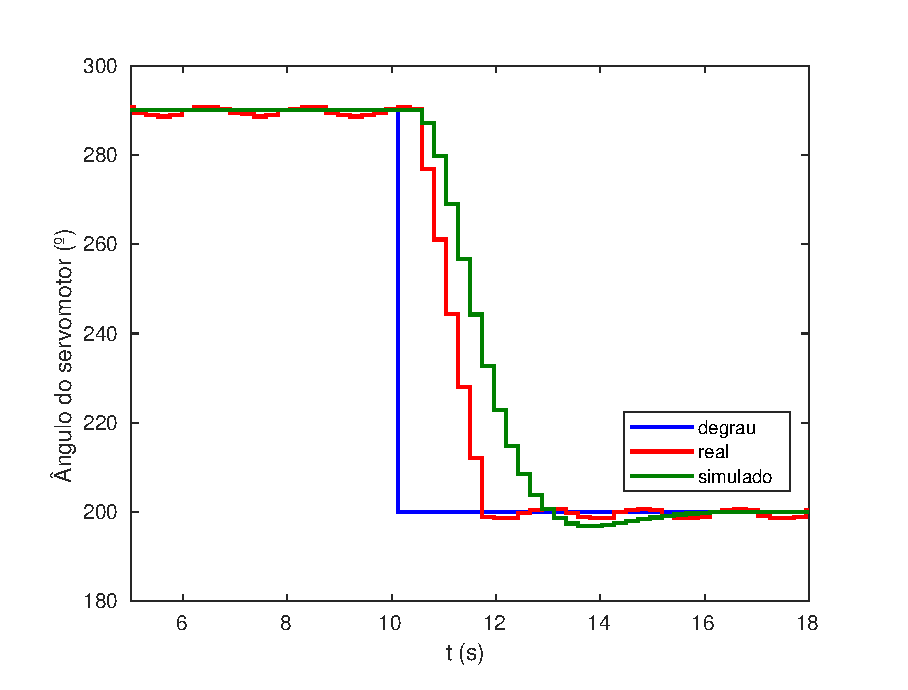
\includegraphics[width = .9\columnwidth]{Imagens/base_mf_simul}
    \caption{Base}
    \fonte{Do autor}
    \label{fig:base_mf_simul}
  \end{subfigure}%
  \begin{subfigure}{.5\textwidth}
    \centering
    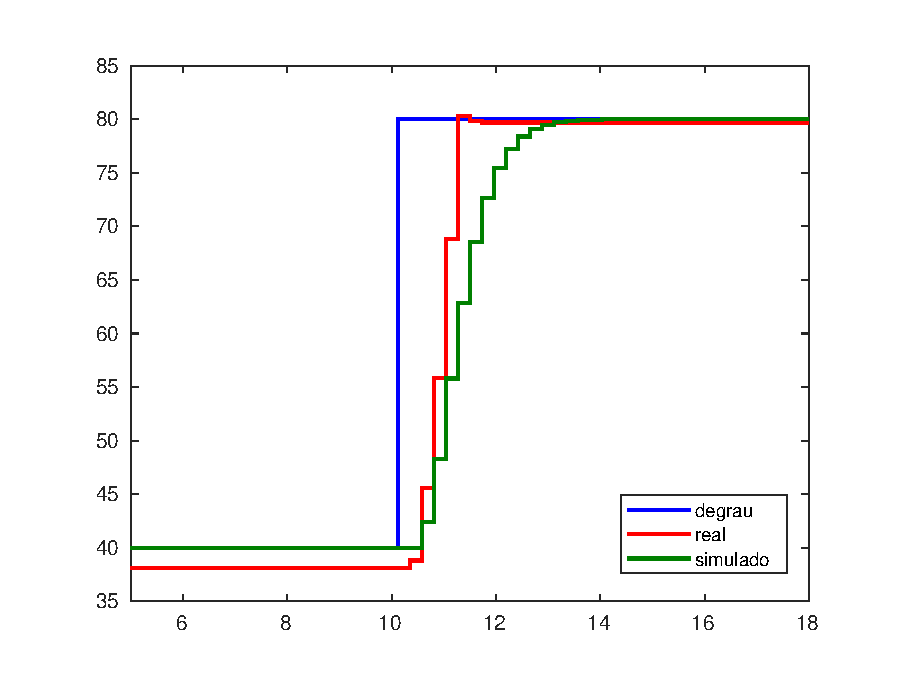
\includegraphics[width = .9\columnwidth]{Imagens/shoulder_mf_simul}
    \caption{Ombro}
    \fonte{Do autor}
    \label{fig:shoulder_mf_simul}
  \end{subfigure}%
  
\end{figure}

\begin{figure}[h!]\ContinuedFloat
  \begin{subfigure}{\textwidth}
    \centering
    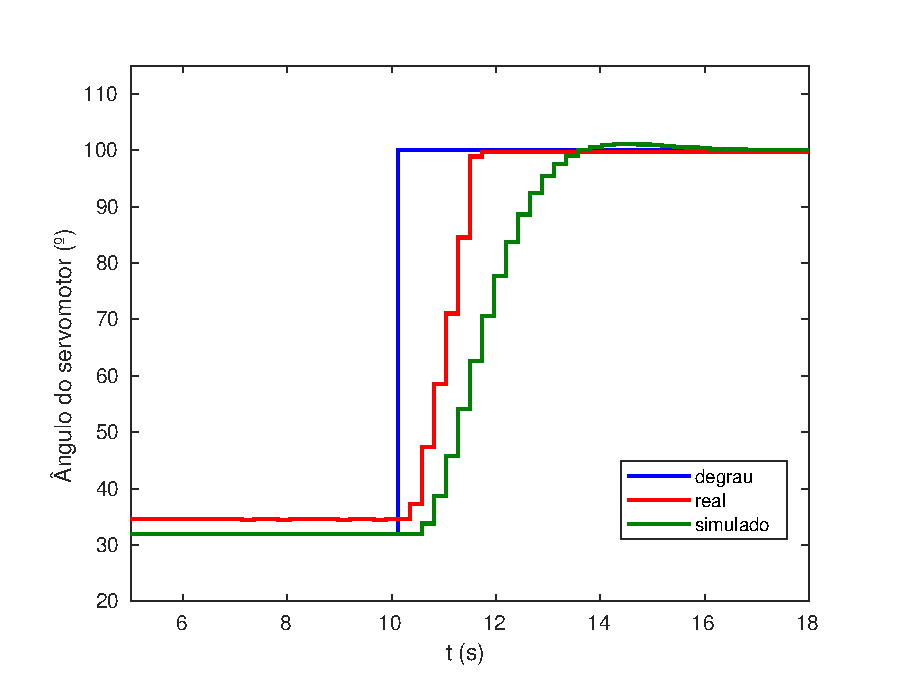
\includegraphics[width = 0.55\columnwidth]{Imagens/forearm_mf_simul}
    \caption{Cotovelo}
    \fonte{Do autor}
    \label{fig:forearm_mf_simul}
  \end{subfigure}%
  \caption{Gráficos das respostas ao degrau em malha fechada - HIL Fase 1}
  \label{fig:malhaFechadaHil1}
\end{figure}

%Com o primeiro controlador projetado para a base e para o cotovelo, ao fechar a malha, a resposta não apresentava
%sobresinal como mostrado na \autoref{fig:base_mf_simul} e na \autoref{fig:forearm_mf_simul}. Apesar disso,
%ao passar para o domínio discreto, o controlador passava a ter um zero não mínimo. E como foi citado 
%anteriormente, o zero não mínimo é um comportamento indesejado para o sistema, por esse motivo, o controlador
%de ambas as juntas foi alterado.

Nota-se na \autoref{fig:malhaFechadaHil1} que as respostas obtidas em malha fechada possuem uma dinâmica mais lenta,
isso se deve à não necessidade de uma resposta rápida, mas sim, à necessidade de uma transição mais suave. Outro fator
levado em consideração ao fechar a malha foi a obtenção do erro em estado estacionário igual a zero. Em malha aberta, a base 
apresentava uma variação em torno do estado estacionário infindável, ao fechar a malha essa variação foi corrigida quando o
sistema entra em estado estacionário.

\section{Fase 2 da técnica HIL - Planta simulada, controlador real}
\markright{\thesection ~~~ Fase 2 da técnica HIL}

Como o sinal da resposta da planta é amostrado periodicamente pela placa de aquisição de dados do
computador e pela \textit{Raspberry Pi}, torna-se necessária a discretização do controlador e da planta simulada. A 
discretização foi feita através do comando \textit{c2d( )} do \textit{Matlab} utilizando um segurador de 
ordem zero e com um tempo de amostragem de $0,23s$. O resultado da discretização para as juntas e os respectivos
controladores segue.
Para a base:
\begin{equation}
  \begin{gathered}
    G(z) = \frac{0,8273z - 0,6543}{z^2 - 0,9515z + 0,1245} \quad \text{e} \quad C(z) = \frac{0,152z + 0,032}{z - 1}
  \end{gathered}
  \label{eq:base_discrete}
\end{equation}
para o ombro:
\begin{equation}
  \begin{gathered}
    G(z) = \frac{0,3876z - 0,198}{z^2 - 0,5515z + 0,1393} \quad \text{e} \quad C(z) = \frac{0,1572z + 0,06513}{z - 1}
  \end{gathered}
  \label{eq:shoulder_discrete}
\end{equation}
para o cotovelo:
\begin{equation}
  \begin{gathered}
   G(z) = \frac{0,8273z - 0,6543}{z^2 - 0,9515z + 0,1245} \quad \text{e} \quad C(z) = \frac{0,152z + 0,032}{z - 1}
  \end{gathered}
  \label{eq:forearm_discrete}
\end{equation}

O próximo passo foi a obtenção da equação de diferenças para cada uma das plantas e
controladores. Para isso, foi feito o seguinte procedimento para o modelo da base e seu respectivo controlador:

\begin{equation*}
  \begin{gathered}
    G(z) = \frac{0,8273z - 0,6543}{z^2 - 0,9515z + 0,1245} \\[0.5cm]
    \frac{Y(z)}{U(z)} = \frac{0,8273z - 0,6543}{z^2 - 0,9515z + 0,1245}\\[0.5cm]
    \frac{Y(z)}{U(z)} = \frac{0,8273/z - 0,6543/z^2}{1 - 0,9515/z + 0,1245/z^2}\\[0.5cm]
    Y(z) - \frac{0,9515}{z} \;Y(z) + \frac{0,1245}{z^2} \;Y(z) = \frac{0,8273}{z} \;U(z) - \frac{0,6543}{z^2} \;U(z)
  \end{gathered}
  \label{eq:base_plant_diffEqIntro}
\end{equation*}
\begin{equation}
  \begin{gathered}
    y(k) = 0,8273 \;u(k-1) - 0,6543 \;u(k-2) + 0,9515 \;y(k-1) - 0,1245 \;y(k-2)
  \end{gathered}
  \label{eq:base_plant_diffEq}
\end{equation}

\begin{equation*}
  \begin{gathered}
    C(z) = \frac{0,152z + 0,032}{z - 1}\\[0.5cm]
    \frac{U(z)}{E(z)} = \frac{0,152z + 0,032}{z - 1}\\[0.5cm]
    \frac{U(z)}{E(z)} = \frac{0,152 + 0,032/z}{1 - 1/z}\\[0.5cm]
    U(z) - \frac{U(z)}{z} = 0,152\;E(z) + \frac{0,032}{z}\;E(z)\\[0.5cm]
  \end{gathered}
  \label{eq:base_ctrl_diffEqIntro}
\end{equation*}
\begin{equation}
  \begin{gathered}
    u(k) = u(k-1) + 0,152\; e(k) + 0,032 \;e(k-1)
  \end{gathered}
  \label{eq:base_ctrl_diffEq}
\end{equation}

O procedimento elucidado é repetido para os modelos e controladores do ombro \eqref{eq:shouder_plant_diffEq} - \eqref{eq:shouder_ctrl_diffEq} 
e do cotovelo \eqref{eq:forearm_plant_diffEq} - \eqref{eq:forearm_ctrl_diffEq}, resultando nos seguintes pares de equações a diferenças:
\begin{equation}
  \begin{gathered}
    y(k) = 0,3876 u(k-1) + 0,198 u(k-2) + 0,5515 y(k-1) - 0,1393 y(k-2)
  \end{gathered}
  \label{eq:shouder_plant_diffEq}
\end{equation}
\begin{equation}
  \begin{gathered}
    u(k) = u(k-1) + 0,1572  e(k) + 0,06513 e(k-1)
  \end{gathered}
  \label{eq:shouder_ctrl_diffEq}
\end{equation}
\begin{equation}
  \begin{gathered}
    y(k) = 0,8273 u(k-1) - 0,6543 u(k-2) + 0,9515y(k-1) - 0,1245y(k-2)
  \end{gathered}
  \label{eq:forearm_plant_diffEq}
\end{equation}
\begin{equation}
  \begin{gathered}
    u(k) = u(k-1) + 0,152 e(k) + 0,032 e(k-1)
  \end{gathered}
  \label{eq:forearm_ctrl_diffEq}
\end{equation}

% para a planta do ombro:
% 
% \begin{equation*}
%   \begin{gathered}
%     G(z) = \frac{0,3876 z + 0,198}{z^2 - 0,5515 z + 0,1393} \\[0.5cm]
%     \frac{Y(z)}{U(z)} = \frac{0,3876 z + 0,198}{z^2 - 0,5515 z + 0,1393}\\[0.5cm]
%     \frac{Y(z)}{U(z)} = \frac{0,3876/z + 0,198/z^2}{1 - 0,5515/z + 0,1393/z^2}\\[0.5cm]
%     Y(z) - \frac{0,5515}{z} \;Y(z) + \frac{0,1393}{z^2} \;Y(z) = \frac{0,3876}{z} \;U(z) + \frac{0,198}{z^2} \;U(z)
%   \end{gathered}
%   \label{eq:shouder_plant_diffEqIntro}
% \end{equation*}
% \begin{equation}
%   \begin{gathered}
%     y(k) = 0,3876 \;u(k-1) + 0,198 \;u(k-2) + 0,5515 \;y(k-1) - 0,1393 \;y(k-2)
%   \end{gathered}
%   \label{eq:shouder_plant_diffEq}
% \end{equation}
% para o controlador do ombro:
% 
% \begin{equation*}
%   \begin{gathered}
%     C(z) = \frac{0,1572 z + 0,06513}{z - 1}\\[0.5cm]
%     \frac{U(z)}{E(z)} = \frac{0,1572 z + 0,06513}{z - 1}\\[0.5cm]
%     \frac{U(z)}{E(z)} = \frac{0,1572 + 0,06513/z}{1 - 1/z}\\[0.5cm]
%     U(z) - \frac{U(z)}{z} = 0,1572 \;E(z) + \frac{0,06513}{z}\;E(z)\\[0.5cm]
%   \end{gathered}
%   \label{eq:shouder_ctrl_diffEqIntro}
% \end{equation*}
% \begin{equation}
%   \begin{gathered}
%     u(k) = u(k-1) + 0,1572 \; e(k) + 0,06513 \;e(k-1)
%   \end{gathered}
%   \label{eq:shouder_ctrl_diffEq}
% \end{equation}
% para a planta do cotovelo:
% 
% \begin{equation*}
%   \begin{gathered}
%     G(z) = \frac{0,8273z - 0,6543}{z^2 - 0,9515z + 0,1245} \\[0.5cm]
%     \frac{Y(z)}{U(z)} = \frac{0,8273z - 0,6543}{z^2 - 0,9515z + 0,1245}\\[0.5cm]
%     \frac{Y(z)}{U(z)} = \frac{0,8273/z - 0,6543/z^2}{1 - 0,9515/z + 0,1245/z^2}\\[0.5cm]
%     Y(z) - \frac{0,9515}{z} \;Y(z) + \frac{0,1245}{z^2} \;Y(z) = \frac{0,8273}{z} \;U(z) - \frac{0,6543}{z^2} \;U(z)
%   \end{gathered}
%   \label{eq:forearm_plant_diffEqIntro}
% \end{equation*}
% \begin{equation}
%   \begin{gathered}
%     y(k) = 0,8273 \;u(k-1) - 0,6543 \;u(k-2) + 0,9515 \;y(k-1) - 0,1245 \;y(k-2)
%   \end{gathered}
%   \label{eq:forearm_plant_diffEq}
% \end{equation}
% para o controlador do cotovelo:
% 
% \begin{equation*}
%   \begin{gathered}
%     C(z) = \frac{0,152z + 0,032}{z - 1}\\[0.5cm]
%     \frac{U(z)}{E(z)} = \frac{0,152z + 0,032}{z - 1}\\[0.5cm]
%     \frac{U(z)}{E(z)} = \frac{0,152 + 0,032/z}{1 - 1/z}\\[0.5cm]
%     U(z) - \frac{U(z)}{z} = 0,152\;E(z) + \frac{0,032}{z}\;E(z)\\[0.5cm]
%   \end{gathered}
%   \label{eq:forearm_ctrl_diffEqIntro}
% \end{equation*}
% \begin{equation}
%   \begin{gathered}
%     u(k) = u(k-1) + 0,152\; e(k) + 0,032 \;e(k-1)
%   \end{gathered}
%   \label{eq:forearm_ctrl_diffEq}
% \end{equation}

Determinadas as equações a diferenças, foi necessário realizar a montagem conforme a 
\autoref{fig:solucaoModelo}, isto é, configurar a conexão UART entre o computador e a 
\textit{Raspberry Pi}, e escrever o código em \textit{Python} para a planta simulada e
para o controlador que passou a rodar na \textit{Raspberry Pi} \cite{lelis_hil2}. Com isso,
a parte referente à simulação da planta ficou conforme o que segue: \\

\begin{lstlisting}[language=Python]
	# BASE - Funcao de transferencia da planta
	y_k[0] = 0.8273*u_k_delay[0] - 0.6543*u_k_delay_2[0]
	  + 0.9515*y_k_delay[0] - 0.1245*y_k_delay_2[0]

	# SHOULDER - Funcao de transferencia da planta
	y_k[1] = 0.3876*u_k_delay[1] + 0.198*u_k_delay_2[1]
	  + 0.5515*y_k_delay[1] - 0.1393*y_k_delay_2[1];

	# FOREARM - Funcao de transferencia da planta
	y_k[2] = 0.8273*u_k_delay[2] - 0.6543*u_k_delay_2[2]
	  + 0.9515*y_k_delay[2] - 0.1245*y_k_delay_2[2];
\end{lstlisting}
e do lado do controlador na \textit{Raspberry Pi}: \\

\begin{lstlisting}[language=Python]
	# BASE - Funcao de transferencia do controlador
	u_k[0] = u_k_delay[0] + 0.152*e_k[0] + 0.032*e_k_delay[0]

	# SHOULDER - Funcao de transferencia do controlador
	u_k[1] = u_k_delay[1] + 0.1572*e_k[1] + 0.06513*e_k_delay[1]

	# FOREARM - Funcao de transferencia do controlador
	u_k[2] = u_k_delay[2] + 0.152*e_k[2] + 0.032*e_k_delay[2]
\end{lstlisting}

Foram aplicadas as mesmas referências em degrau da primeira fase da técnica HIL para 
cada uma das plantas simuladas. Assim, as saídas obtidas ao longo do tempo para 
a fase 2 da técnica HIL são apresentadas nas Figuras \ref{fig:base_hilFase2}, 
\ref{fig:shoulder_hilFase2} e \ref{fig:forearm_hilFase2}.

\newpage

\begin{figure}[h!]
  
  \centering
  \begin{subfigure}{.5\textwidth}
    \centering
    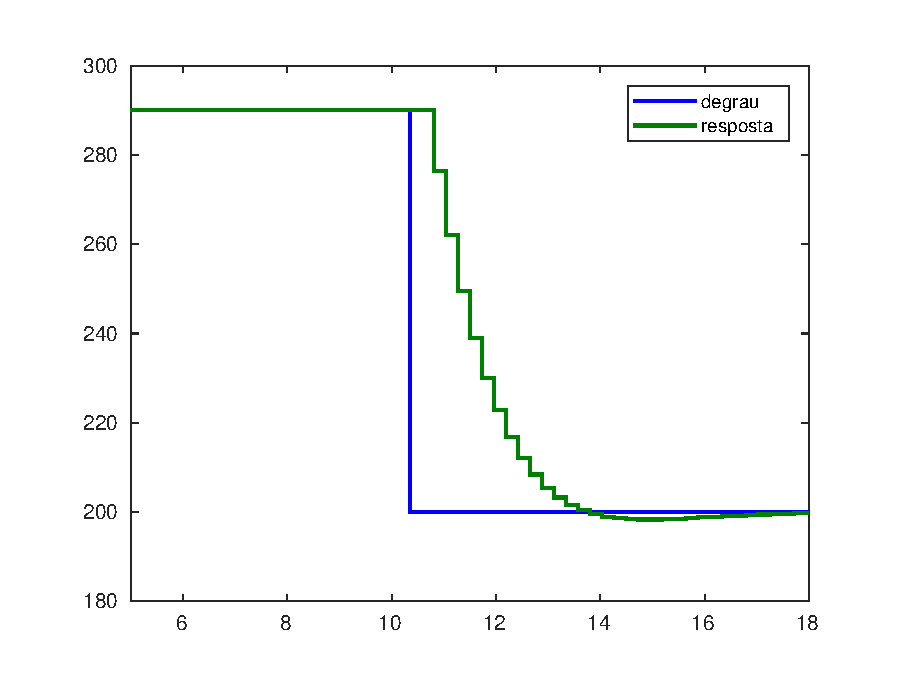
\includegraphics[width = 1\columnwidth]{Imagens/base_hilFase2}
    \caption{Base}
    \fonte{Do autor}
    \label{fig:base_hilFase2}
  \end{subfigure}%
  \begin{subfigure}{.5\textwidth}
    \centering
    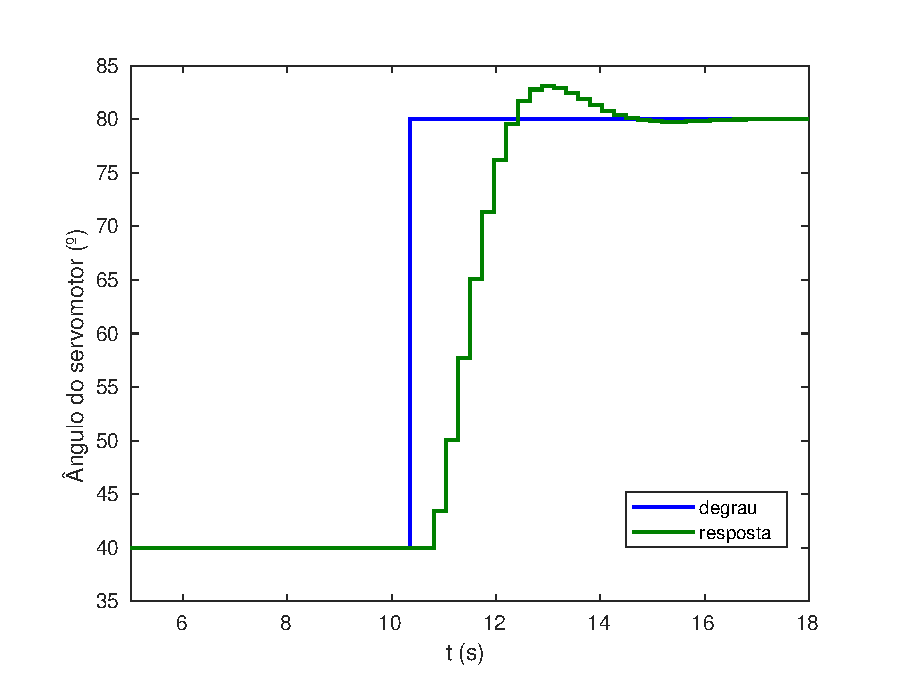
\includegraphics[width = 1\columnwidth]{Imagens/shoulder_hilFase2}
    \caption{Ombro}
    \fonte{Do autor}
    \label{fig:shoulder_hilFase2}
  \end{subfigure}%
  \\[5ex]
  \begin{subfigure}{\textwidth}
    \centering
    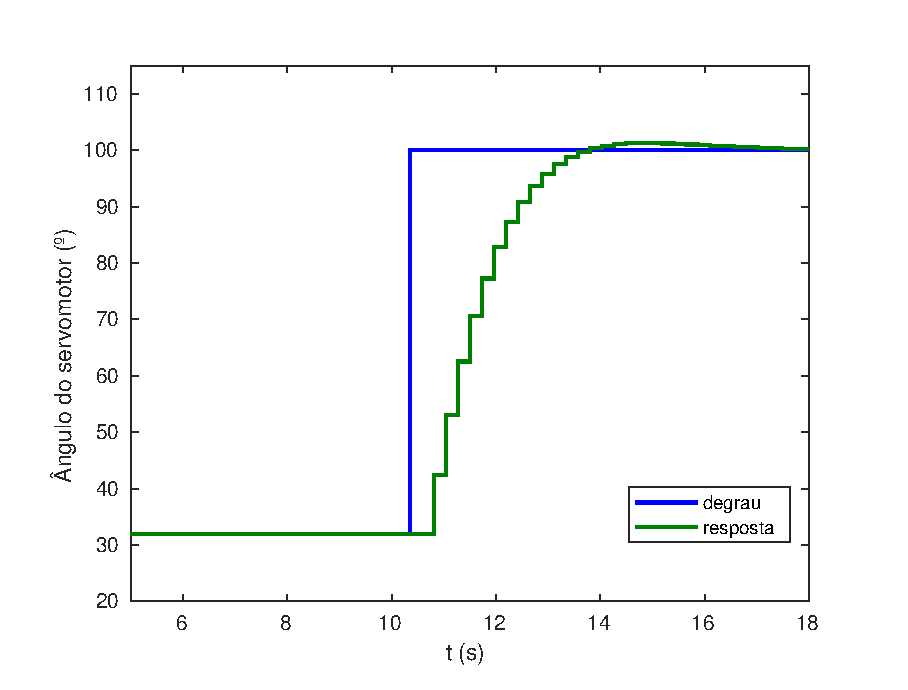
\includegraphics[width = 0.55\columnwidth]{Imagens/forearm_hilFase2}
    \caption{Cotovelo}
    \fonte{Do autor}
    \label{fig:forearm_hilFase2}
  \end{subfigure}%
  \caption{Gráficos das respostas ao degrau em malha fechada - HIL Fase 2}
  \label{fig:hilFase2}

\end{figure}

\section{Fase 3 da técnica HIL - Planta e controlador reais}
\markright{\thesection ~~~ Fase 3 da técnica HIL}

A última etapa da técnica HIL consiste em conectar o controlador implementado e validado 
na \textit{Raspberry Pi} e conectá-lo à malha de controle da planta do
manipulador, conforme a \autoref{fig:solucaoPlanta}. Além disso, foi necessário configurar
um ambiente de comunicação serial UART com os servomotores do manipulador. Para isso, uma
biblioteca em \textit{Python} foi utilizada. A parte do código referente à geração do sinal 
de controle é apresentada abaixo, sendo que o código completo encontra-se disponível 
em \cite{lelis_hil3}.\\[2cm]

\begin{lstlisting}[language=Python]
	def get_U_k(self, y_k):
		# Calcula lei de controle
		r_k = self.reference
		e_k = r_k - y_k
		
		# Controle de posicao
		u_k = self.u_k_delay + self.Kp*e_k + self.Ki*self.e_k_delay
		
		return u_k, e_k
\end{lstlisting}

Foram aplicadas referências em degrau, mas com leves diferenças para as amplitudes
das etapas da técnica HIL anteriores. Desse modo, as saídas obtidas ao longo do 
tempo para a fase 3 da técnica HIL são mostradas nas Figuras \ref{fig:base_hilFase3}, 
\ref{fig:shoulder_hilFase3} e \ref{fig:forearm_hilFase3}.

\begin{figure}[h!]
  
  \centering
  \begin{subfigure}{.5\textwidth}
    \centering
    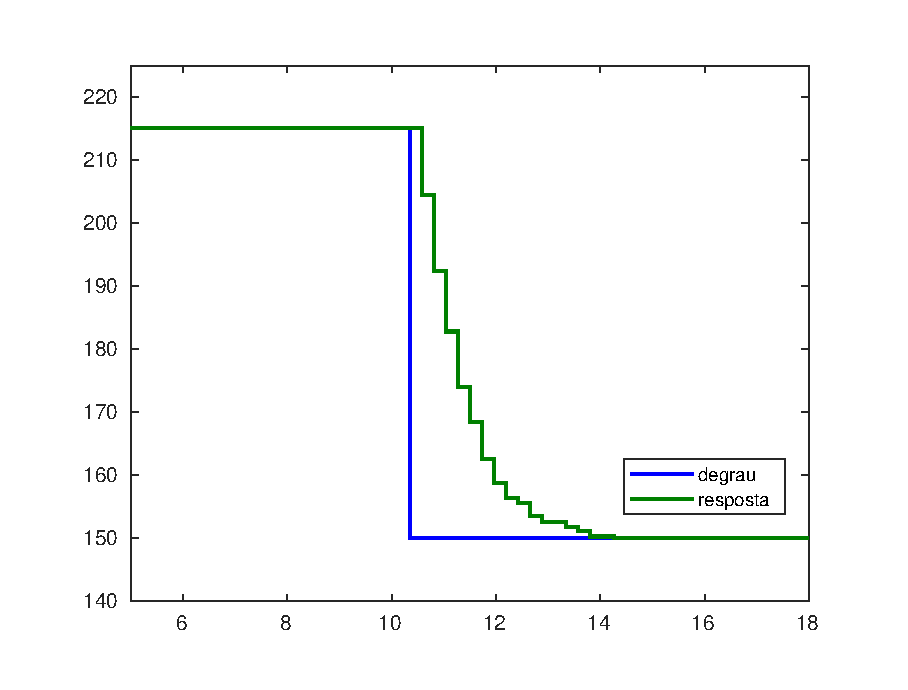
\includegraphics[width = 1\columnwidth]{Imagens/base_hilFase3}
    \caption{Base}
    \fonte{Do autor}
    \label{fig:base_hilFase3}
  \end{subfigure}%
  \begin{subfigure}{.5\textwidth}
    \centering
    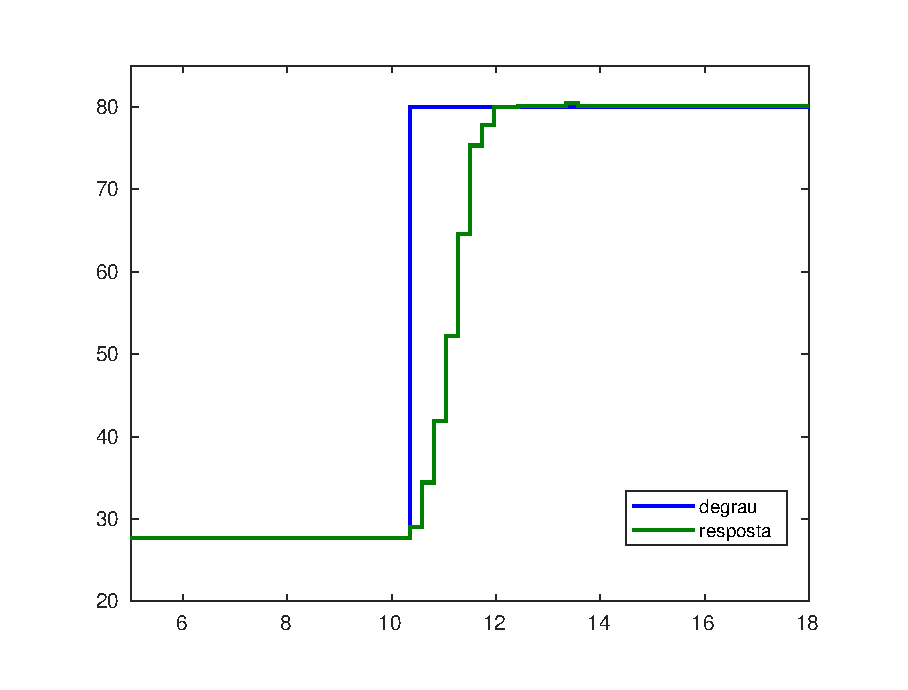
\includegraphics[width = 1\columnwidth]{Imagens/shoulder_hilFase3}
    \caption{Ombro}
    \fonte{Do autor}
    \label{fig:shoulder_hilFase3}
  \end{subfigure}%
  \\
  \begin{subfigure}{\textwidth}
    \centering
    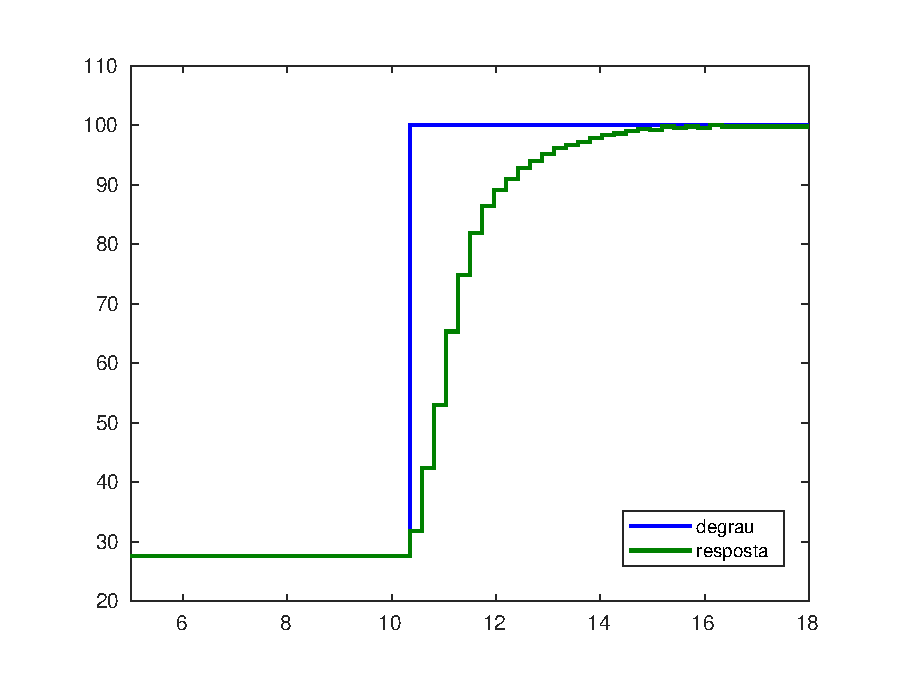
\includegraphics[width = 0.5\columnwidth]{Imagens/forearm_hilFase3}
    \caption{Cotovelo}
    \fonte{Do autor}
    \label{fig:forearm_hilFase3}
  \end{subfigure}%
  \caption{Gráficos das respostas ao degrau em malha fechada - HIL Fase 3}
  \label{fig:hilFase3} 

\end{figure}

\section{Resumo do Capítulo}
\markright{\thesection ~~~ Resultados}

Este capítulo apresentou os resultados alcançados no projeto, apresentando a memória de cálculo,
explicitando como o sistema foi iplementado e expondo os resultados por meio dos gráficos. No próximo
capítulo são apresentadas as conclusões do projeto, como os resultados estão relacionados, são expostos e também 
os problemas encontrados. Além disso, são tecidas algumas sugestões para uma futura evolução do projeto.


\clearpage
\chapter{Conclusão}
%\markboth{\thechapter ~~~ Conclusão}{}
%\label{revBib}

O controle de trajetória de uma manipulador robótico visa configurar o comportamento das juntas de tal 
forma que a ferramenta de trabalho siga uma trajeto de referência.
As maneiras mais usuais de se modelar o comportamento de juntas robóticas são por meio da metodologia de
\textit{Denavit-Hartenberg} e das equações de \textit{Euler-Lagrange}, além do modelo de juntas independentes.
No presente projeto, a modelagem foi tratada das duas maneiras
e o projeto do controlador foi realizado pelo método do lugar das raízes. A sintonia e validação da estratégia de controle
foi realizada por meio do uso da técnica HIL.

A técnica HIL, que consiste em inserir um dispositivo físico na malha de controle simulada, foi dividida
em três etapas neste projeto. O resultado obtido em cada uma das etapas foi exposto através
dos gráficos com o objetivo de que o padrão se repetisse entre as etapas. Além disso, a sintonia
e validação da estratégia de controle para a planta em questão é fundamental para o êxito da 
conclusão do projeto.

Analisando o exposto no capítulo anterior, observa-se que as considerações feitas para simplificar
a modelagem \textit{Denavit-Hartenberg} e as equações de \textit{Euler-Lagrange} tornaram o desenvolvimento
da solução para o modelo da planta fisicamente inviável. A solução mais coerente encontrada foi o ensaio 
em malha aberta para a obtenção do modelo de cada junta do manipulador, seguido do controle de junta independente.

Os experimentos demonstraram que a modelagem do manipulador teve um resultado coerente com a planta real, sendo que as curvas
de resposta ao degrau se sobrepuseram e os parâmetros de tempo de acomodação e máximo sobressinal ficaram bastante similares como desejado. 
O projeto de controle pelo método do lugar das raízes teve como resultado um controlador que tornou a dinâmica da 
planta mais lenta. Por outro lado, o controlador PI fez o sistema ficar mais robusto, rejeitando distúrbios ao fechar
a malha além de tornar a transição dos estados mais suave (é possível notar a diferença entre as respostas apresentadas na 
\autoref{fig:ensaioMalhaAberta} e na \autoref{fig:hilFase3}). Além disso, as respostas ao degrau dos modelos obtidos
foram coerentes e apresentaram o mesmo comportamento em todas as etapas do método HIL. Assim, a sintonia e
validação da estratégia de controle foi realizada com êxito.

Por fim, o desafio futuro envolve tanto a planta do manipulador quanto a configuração \textit{Hardware in the loop}. Para o
manipulador é necessário reduzir ou remover a trepidação observada principalmente na base. Essa trepidação foi reduzida ao
validar a estratégia de controle (conforme a \autoref{fig:hilFase3} mostra), mas ela ainda perdura.
A implementação de outras estratégias de controle pode auxiliar na redução da trepidação das juntas e aumento da robustez do sistema.
Em relação à técnica HIL, é de grande importância optar por um \textit{hardware} de tempo real, o que não foi atendido com a \textit{Raspberry Pi}.
A solução mais coerente seria modificar o \textit{kernel} \textit{Linux} da \textit{Raspberry Pi} para tornar o tempo 
de resposta aos eventos um tempo pré-definido.





\addcontentsline{toc}{chapter}{Referências Bibliográficas}
\bibliographystyle{abntex2-alf}
\bibliography{Monografia}

\begin{anexosenv}
\partanexos

\chapter{Obtenção do modelo através da convenção de \textit{Denavit-Hartenberg} e equações de \textit{Euler-Lagrange}}
\label{anexo:denHatEulerLagr}

\begin{lstlisting}[language=Matlab]
clc;
close all;

% ---------------------- 1) DENAVIT - HATENBERG ------------------------
% Rodar o Matlab com um usuario com alto privilegio
% 1.1) Carregando a matriz de Denavit-Hatenberg

dh = [
    0,  0,      0,      0;
    0,  0.085,  0.065,  -pi/2;
    0,  0,      0.172,  0;
    0,  0,      0.235,  0];
dh_representation = SerialLink(dh)

% Carregando angulos iniciais das juntas (radianos)
q = [0, 0, 0, 0]

% Representacao grafica do manipulador
dh_representation.plot(q)
dh_representation.teach

% 1.2) Matrizes homogeneas

% Especificidades do manipulador em estudo
syms theta_0 theta_1 theta_2 theta_3;

alpha_0 = 0;
alpha_1 = -pi/2;
alpha_2 = 0;
alpha_3 = 0;

a0 = 0;
a1 = 0.065;
a2 = 0.172;
a3 = 0.235;

d0 = 0;
d1 = 0.085;
d2 = 0;
d3 = 0;

syms s0 c0 s1 c1 s2 c2 s3 c3
% Usar para exibir resultado em funcao de theta (resultado simbolico)
A_0 =   [
            [c0     -s0*1    s0*0   a0*c0];
            [s0     c0*1     -c0*0  a0*s0];
            [0      0        1      d0   ];
            [0      0        0      1    ];
        ];
A_1 =   [
            [c1     -s1*0    s1*-1   a1*c1];
            [s1     c1*0     -c1*-1  a1*s1];
            [0      -1        0      d1   ];
            [0      0         0      1    ];
        ];
A_2 =   [
            [c2     -s2*1	s2*0   a2*c2];
            [s2     c2*1     -c2*0  a2*s2];
            [0      0        1      d2   ];
            [0      0        0      1    ];
        ];
A_3 =   [
            [c3     -s3*1    s3*0   a3*c3];
            [s3     c3*1     -c3*0  a3*s3];
            [0      0        1      d3   ];
            [0      0        0      1    ];
        ];

% Matriz homogenea resultante - z0 = [0 0 1]' e o0 = [0 0 0]'
T_0_1 = A_1;
T_0_2 = A_1*A_2;
T_0_3 = A_1*A_2*A_3;
Tresp = vpa(T_0_3,3);

R_1 = T_0_1(1:3,1:3);
R_2 = T_0_2(1:3,1:3);
R_3 = T_0_3(1:3,1:3);

% -------------------- 2) EULER - LAGRANGE -----------------------------

% 2.1) Jacobiano

% z_i = terceira coluna / o_i = quarta coluna
z_0 = A_0(1:3,3);
o_0 = A_0(1:3,4);

z_1 = T_0_1(1:3,3);
o_1 = T_0_1(1:3,4);

z_2 = T_0_2(1:3,3);
o_2 = T_0_2(1:3,4);

z_3 = T_0_3(1:3,3);
o_3 = T_0_3(1:3,4);

% Jacobianos para as juntas revolutas (SPONG)
J_parc_1 =  [
                cross(z_0,(o_3-o_0));
                z_0;
            ];
J_parc_2 =  [
                cross(z_1,(o_3-o_1));
                z_1;
            ];
J_parc_3 =  [
                cross(z_2,(o_3-o_2));
                z_2;
            ];

% Resultados
J_1 =   [
            J_parc_1     zeros(6,2);
        ];
J_2 =   [
            J_parc_1     J_parc_2     zeros(6,1);
        ];
J_3 =   [
            J_parc_1     J_parc_2     J_parc_3;
        ];

J_1 = vpa(J_1,3);
J_2 = vpa(J_2,3);
J_3 = vpa(J_3,3)

% ----------------------------- Matriz D(q) ---------------------------

% Elbow manipulator / articulated / revolute / anthropomorphic / RRR

% As tres primeiras linhas da matriz J correspondem a velocidade 
% linear e as tres ultimas a velocidade angular
J_v1 = J_1(1:3,:);
J_w1 = J_1(4:6,:);
J_v2 = J_2(1:3,:);
J_w2 = J_2(4:6,:);
J_v3 = J_3(1:3,:);
J_w3 = J_3(4:6,:);

% Barra de comprimento L e massa m (Eixo de rotacao no fim da barra)
% Iy = Iz = 1/3*m*L^2, onde o eixo x eh o unico paralelo a barra

% Caso a distribuicao de massa do corpo seja simetrica em relacao a
% estrutura do corpo, entao os produtos cruzados de inercia sao 
% identicos a zero
m_motor = .055;
m_elo = .010;
Raio_1 = .085;
g = 9.8;
L_1 = .085;
L_2 = .172;
L_3 = .235;

m_1 = m_elo;
m_2 = m_elo+m_motor*2;
m_3 = m_elo+m_motor*4;

I_1 =   [
            0               0               0;
            0               0               0;
            0               0               1/2*m_1*Raio_1^2;
        ]
I_2 =   [
            0               0               0;
            0               0               0;
            0               0               1/3*m_2*L_2^2;
        ]
I_3 =   [
            0               0               0;
            0               0               0;
            0               0               1/3*m_3*L_3^2;
        ]

D1 = m_1*(J_v1).'*J_v1+J_w1.'*R_1*I_1*R_1.'*J_w1;
D2 = m_2*(J_v2).'*J_v2+J_w2.'*R_2*I_2*R_2.'*J_w2;
D3 = m_3*(J_v3).'*J_v3+J_w3.'*R_3*I_3*R_3.'*J_w3;

D = vpa(D1,3) + vpa(D2,3) + vpa(D3,3);

% -------------------- Simbolos de Christoffel -----------------------

% Derivadas: sen(x) = cos(x) / cos(x) = -sen(x)

syms theta_1 theta_2 theta_3
D_11 = (0.065*sin(theta_1) + 0.17*cos(theta_2)*sin(theta_1) + 
    0.24*cos(theta_2)*cos(theta_3)*sin(theta_1) - 
    0.24*sin(theta_1)*sin(theta_2)*sin(theta_3))*(0.015*sin(theta_1)
    + 0.04*cos(theta_2)*sin(theta_1) +
    0.054*cos(theta_2)*cos(theta_3)*sin(theta_1) - 
    0.054*sin(theta_1)*sin(theta_2)*sin(theta_3)) +
    (0.065*sin(theta_1) + 0.17*cos(theta_2)*sin(theta_1) +
    0.24*cos(theta_2)*cos(theta_3)*sin(theta_1) - 
    0.24*sin(theta_1)*sin(theta_2)*sin(theta_3))*(7.8e-3*sin(theta_1)
    + 0.021*cos(theta_2)*sin(theta_1) +
    0.028*cos(theta_2)*cos(theta_3)*sin(theta_1) - 
    0.028*sin(theta_1)*sin(theta_2)*sin(theta_3)) +
    (0.065*cos(theta_1) + 0.17*cos(theta_1)*cos(theta_2) +
    0.24*cos(theta_1)*cos(theta_2)*cos(theta_3) - 
    0.24*cos(theta_1)*sin(theta_2)*sin(theta_3))*(6.5e-4*cos(theta_1)
    + 1.7e-3*cos(theta_1)*cos(theta_2) +
    2.4e-3*cos(theta_1)*cos(theta_2)*cos(theta_3) - 
    2.4e-3*cos(theta_1)*sin(theta_2)*sin(theta_3)) +
    (0.065*cos(theta_1) + 0.17*cos(theta_1)*cos(theta_2) +
    0.24*cos(theta_1)*cos(theta_2)*cos(theta_3) - 
    0.24*cos(theta_1)*sin(theta_2)*sin(theta_3))*(0.015*cos(theta_1)
    + 0.04*cos(theta_1)*cos(theta_2) +
    0.054*cos(theta_1)*cos(theta_2)*cos(theta_3) - 
    0.054*cos(theta_1)*sin(theta_2)*sin(theta_3)) +
    (0.065*cos(theta_1) + 0.17*cos(theta_1)*cos(theta_2) +
    0.24*cos(theta_1)*cos(theta_2)*cos(theta_3) - 
    0.24*cos(theta_1)*sin(theta_2)*sin(theta_3))*(7.8e-3*cos(theta_1)
    + 0.021*cos(theta_1)*cos(theta_2) +
    0.028*cos(theta_1)*cos(theta_2)*cos(theta_3) - 
    0.028*cos(theta_1)*sin(theta_2)*sin(theta_3)) +
    (6.5e-4*sin(theta_1) + 1.7e-3*cos(theta_2)*sin(theta_1) +
    2.4e-3*cos(theta_2)*cos(theta_3)*sin(theta_1) - 
    2.4e-3*sin(theta_1)*sin(theta_2)*sin(theta_3))*(0.065*sin(theta_1)
    + 0.17*cos(theta_2)*sin(theta_1) +
    0.24*cos(theta_2)*cos(theta_3)*sin(theta_1) - 
    0.24*sin(theta_1)*sin(theta_2)*sin(theta_3));

D_12 = 1.0*cos(theta_1)*(0.17*sin(theta_2) +
    0.24*cos(theta_2)*sin(theta_3) + 
    0.24*cos(theta_3)*sin(theta_2))*(0.015*sin(theta_1) +
    0.04*cos(theta_2)*sin(theta_1) + 
    0.054*cos(theta_2)*cos(theta_3)*sin(theta_1) -
    0.054*sin(theta_1)*sin(theta_2)*sin(theta_3)) + 
    1.0*cos(theta_1)*(0.17*sin(theta_2) +
    0.24*cos(theta_2)*sin(theta_3) + 
    0.24*cos(theta_3)*sin(theta_2))*(7.8e-3*sin(theta_1) +
    0.021*cos(theta_2)*sin(theta_1) + 
    0.028*cos(theta_2)*cos(theta_3)*sin(theta_1) -
    0.028*sin(theta_1)*sin(theta_2)*sin(theta_3)) - 
    1.0*sin(theta_1)*(0.17*sin(theta_2) +
    0.24*cos(theta_2)*sin(theta_3) + 
    0.24*cos(theta_3)*sin(theta_2))*(0.015*cos(theta_1) +
    0.04*cos(theta_1)*cos(theta_2) + 
    0.054*cos(theta_1)*cos(theta_2)*cos(theta_3) -
    0.054*cos(theta_1)*sin(theta_2)*sin(theta_3)) - 
    1.0*sin(theta_1)*(0.17*sin(theta_2) +
    0.24*cos(theta_2)*sin(theta_3) + 
    0.24*cos(theta_3)*sin(theta_2))*(7.8e-3*cos(theta_1) +
    0.021*cos(theta_1)*cos(theta_2) + 
    0.028*cos(theta_1)*cos(theta_2)*cos(theta_3) -
    0.028*cos(theta_1)*sin(theta_2)*sin(theta_3));

D_13 = 1.0*cos(theta_1)*(0.24*cos(theta_2)*sin(theta_3) + 
    0.24*cos(theta_3)*sin(theta_2))*(0.015*sin(theta_1) +
    0.04*cos(theta_2)*sin(theta_1) + 
    0.054*cos(theta_2)*cos(theta_3)*sin(theta_1) -
    0.054*sin(theta_1)*sin(theta_2)*sin(theta_3)) - 
    1.0*sin(theta_1)*(0.24*cos(theta_2)*sin(theta_3) +
    0.24*cos(theta_3)*sin(theta_2))*(0.015*cos(theta_1) + 
    0.04*cos(theta_1)*cos(theta_2) +
    0.054*cos(theta_1)*cos(theta_2)*cos(theta_3) - 
    0.054*cos(theta_1)*sin(theta_2)*sin(theta_3));

D_21 = 0.35*cos(theta_1)*(0.17*sin(theta_2) +
    0.24*cos(theta_2)*sin(theta_3) + 
    0.24*cos(theta_3)*sin(theta_2))*(0.065*sin(theta_1) +
    0.17*cos(theta_2)*sin(theta_1) + 
    0.24*cos(theta_2)*cos(theta_3)*sin(theta_1) -
    0.24*sin(theta_1)*sin(theta_2)*sin(theta_3)) - 
    0.35*sin(theta_1)*(0.17*sin(theta_2) +
    0.24*cos(theta_2)*sin(theta_3) + 
    0.24*cos(theta_3)*sin(theta_2))*(0.065*cos(theta_1) +
    0.17*cos(theta_1)*cos(theta_2) + 
    0.24*cos(theta_1)*cos(theta_2)*cos(theta_3) -
    0.24*cos(theta_1)*sin(theta_2)*sin(theta_3));

D_22 = (0.23*sin(theta_1)*(0.17*cos(theta_2)*sin(theta_1) + 
    0.24*cos(theta_2)*cos(theta_3)*sin(theta_1) -
    0.24*sin(theta_1)*sin(theta_2)*sin(theta_3)) + 
    0.23*cos(theta_1)*(0.17*cos(theta_1)*cos(theta_2) +
    0.24*cos(theta_1)*cos(theta_2)*cos(theta_3) - 
    0.24*cos(theta_1)*sin(theta_2)*sin(theta_3))) *
    (1.0*sin(theta_1)*(0.17*cos(theta_2)*sin(theta_1) +
    0.24*cos(theta_2)*cos(theta_3)*sin(theta_1) -
    0.24*sin(theta_1)*sin(theta_2)*sin(theta_3)) +
    1.0*cos(theta_1)*(0.17*cos(theta_1)*cos(theta_2) +
    0.24*cos(theta_1)*cos(theta_2)*cos(theta_3) - 
    0.24*cos(theta_1)*sin(theta_2)*sin(theta_3))) +
    (0.12*sin(theta_1)*(0.17*cos(theta_2)*sin(theta_1) + 
    0.24*cos(theta_2)*cos(theta_3)*sin(theta_1) -
    0.24*sin(theta_1)*sin(theta_2)*sin(theta_3)) + 
    0.12*cos(theta_1)*(0.17*cos(theta_1)*cos(theta_2) +
    0.24*cos(theta_1)*cos(theta_2)*cos(theta_3) - 
    0.24*cos(theta_1)*sin(theta_2)*sin(theta_3))) *
    (1.0*sin(theta_1)*(0.17*cos(theta_2)*sin(theta_1) + 
    0.24*cos(theta_2)*cos(theta_3)*sin(theta_1) -
    0.24*sin(theta_1)*sin(theta_2)*sin(theta_3)) + 
    1.0*cos(theta_1)*(0.17*cos(theta_1)*cos(theta_2) +
    0.24*cos(theta_1)*cos(theta_2)*cos(theta_3) - 
    0.24*cos(theta_1)*sin(theta_2)*sin(theta_3))) +
    cos(theta_1)^2*(4.2e-3*cos(theta_1)^2 + 
    4.2e-3*sin(theta_1)^2) + 0.35*cos(theta_1)^2*(0.17*sin(theta_2) +
    0.24*cos(theta_2)*sin(theta_3) + 
    0.24*cos(theta_3)*sin(theta_2))^2 +
    1.0*sin(theta_1)^2*(4.2e-3*cos(theta_1)^2 + 
    4.2e-3*sin(theta_1)^2) + cos(theta_1)^2*(1.2e-3*cos(theta_1)^2 +
    1.2e-3*sin(theta_1)^2) + 0.35*sin(theta_1)^2*(0.17*sin(theta_2) +
    0.24*cos(theta_2)*sin(theta_3) + 0.24*cos(theta_3)*sin(theta_2))^2 +
    1.0*sin(theta_1)^2*(1.2e-3*cos(theta_1)^2 + 1.2e-3*sin(theta_1)^2);

D_23 = (0.23*sin(theta_1)*(0.17*cos(theta_2)*sin(theta_1) + 
    0.24*cos(theta_2)*cos(theta_3)*sin(theta_1) -
    0.24*sin(theta_1)*sin(theta_2)*sin(theta_3)) + 
    0.23*cos(theta_1)*(0.17*cos(theta_1)*cos(theta_2) +
    0.24*cos(theta_1)*cos(theta_2)*cos(theta_3) - 
    0.24*cos(theta_1)*sin(theta_2)*sin(theta_3))) *
    (1.0*cos(theta_1)*(0.24*cos(theta_1)*cos(theta_2)*cos(theta_3) - 
    0.24*cos(theta_1)*sin(theta_2)*sin(theta_3)) +
    1.0*sin(theta_1)*(0.24*cos(theta_2)*cos(theta_3)*sin(theta_1) - 
    0.24*sin(theta_1)*sin(theta_2)*sin(theta_3))) +
    cos(theta_1)^2*(4.2e-3*cos(theta_1)^2 + 4.2e-3*sin(theta_1)^2) + 
    1.0*sin(theta_1)^2*(4.2e-3*cos(theta_1)^2 +
    4.2e-3*sin(theta_1)^2) +
    0.23*cos(theta_1)^2*(0.24*cos(theta_2)*sin(theta_3) + 
    0.24*cos(theta_3)*sin(theta_2))*(0.17*sin(theta_2) +
    0.24*cos(theta_2)*sin(theta_3) + 0.24*cos(theta_3)*sin(theta_2)) + 
    0.23*sin(theta_1)^2*(0.24*cos(theta_2)*sin(theta_3) +
    0.24*cos(theta_3)*sin(theta_2))*(0.17*sin(theta_2) + 
    0.24*cos(theta_2)*sin(theta_3) + 0.24*cos(theta_3)*sin(theta_2));

D_31 = 0.23*cos(theta_1)*(0.24*cos(theta_2)*sin(theta_3) + 
    0.24*cos(theta_3)*sin(theta_2))*(0.065*sin(theta_1) +
    0.17*cos(theta_2)*sin(theta_1) + 
    0.24*cos(theta_2)*cos(theta_3)*sin(theta_1) -
    0.24*sin(theta_1)*sin(theta_2)*sin(theta_3)) - 
    0.23*sin(theta_1)*(0.24*cos(theta_2)*sin(theta_3) +
    0.24*cos(theta_3)*sin(theta_2))*(0.065*cos(theta_1) + 
    0.17*cos(theta_1)*cos(theta_2) +
    0.24*cos(theta_1)*cos(theta_2)*cos(theta_3) - 
    0.24*cos(theta_1)*sin(theta_2)*sin(theta_3));

D_32 = 
    (0.23*cos(theta_1)*(0.24*cos(theta_1)*cos(theta_2)*cos(theta_3) - 
    0.24*cos(theta_1)*sin(theta_2)*sin(theta_3)) +
    0.23*sin(theta_1)*(0.24*cos(theta_2)*cos(theta_3)*sin(theta_1) - 
    0.24*sin(theta_1)*sin(theta_2)*sin(theta_3)))*(1.0*sin(theta_1) * 
    (0.17*cos(theta_2)*sin(theta_1) + 
    0.24*cos(theta_2)*cos(theta_3)*sin(theta_1) -
    0.24*sin(theta_1)*sin(theta_2)*sin(theta_3)) + 
    1.0*cos(theta_1)*(0.17*cos(theta_1)*cos(theta_2) +
    0.24*cos(theta_1)*cos(theta_2)*cos(theta_3) - 
    0.24*cos(theta_1)*sin(theta_2)*sin(theta_3))) +
    cos(theta_1)^2*(4.2e-3*cos(theta_1)^2 + 
    4.2e-3*sin(theta_1)^2) +
    1.0*sin(theta_1)^2*(4.2e-3*cos(theta_1)^2 +
    4.2e-3*sin(theta_1)^2) + 
    0.23*cos(theta_1)^2*(0.24*cos(theta_2)*sin(theta_3) +
    0.24*cos(theta_3)*sin(theta_2))*(0.17*sin(theta_2) +
    0.24*cos(theta_2)*sin(theta_3) + 0.24*cos(theta_3)*sin(theta_2)) + 
    0.23*sin(theta_1)^2*(0.24*cos(theta_2)*sin(theta_3) +
    0.24*cos(theta_3)*sin(theta_2))*(0.17*sin(theta_2) +
    0.24*cos(theta_2)*sin(theta_3) + 0.24*cos(theta_3)*sin(theta_2));

D_33 = 0.23*cos(theta_1)^2*(0.24*cos(theta_2)*sin(theta_3) + 
    0.24*cos(theta_3)*sin(theta_2))^2 +
    0.23*sin(theta_1)^2*(0.24*cos(theta_2)*sin(theta_3) + 
    0.24*cos(theta_3)*sin(theta_2))^2 +
    cos(theta_1)^2*(4.2e-3*cos(theta_1)^2 + 
    4.2e-3*sin(theta_1)^2) +
    1.0*sin(theta_1)^2*(4.2e-3*cos(theta_1)^2 +
    4.2e-3*sin(theta_1)^2) + 
    (0.23*cos(theta_1)*(0.24*cos(theta_1)*cos(theta_2)*cos(theta_3) - 
    0.24*cos(theta_1)*sin(theta_2)*sin(theta_3)) + 
    0.23*sin(theta_1)*(0.24*cos(theta_2)*cos(theta_3)*sin(theta_1) - 
    0.24*sin(theta_1)*sin(theta_2)*sin(theta_3))) * 
    (1.0*cos(theta_1)*(0.24*cos(theta_1)*cos(theta_2)*cos(theta_3) - 
    0.24*cos(theta_1)*sin(theta_2)*sin(theta_3)) +
    1.0*sin(theta_1)*(0.24*cos(theta_2)*cos(theta_3)*sin(theta_1) - 
    0.24*sin(theta_1)*sin(theta_2)*sin(theta_3)));

del_d11_theta1 = diff(D_11,theta_1);
del_d11_theta2 = diff(D_11,theta_2);
del_d11_theta3 = diff(D_11,theta_3);

del_d12_theta1 = diff(D_12,theta_1);
del_d12_theta2 = diff(D_12,theta_2);
del_d12_theta3 = diff(D_12,theta_3);

del_d13_theta1 = diff(D_13,theta_1);
del_d13_theta2 = diff(D_13,theta_2);
del_d13_theta3 = diff(D_13,theta_3);

del_d21_theta1 = diff(D_21,theta_1);
del_d21_theta2 = diff(D_21,theta_2);
del_d21_theta3 = diff(D_21,theta_3);

del_d22_theta1 = diff(D_22,theta_1);
del_d22_theta2 = diff(D_22,theta_2);
del_d22_theta3 = diff(D_22,theta_3);

del_d23_theta1 = diff(D_23,theta_1);
del_d23_theta2 = diff(D_23,theta_2);
del_d23_theta3 = diff(D_23,theta_3);

del_d31_theta1 = diff(D_31,theta_1);
del_d31_theta2 = diff(D_31,theta_2);
del_d31_theta3 = diff(D_31,theta_3);

del_d32_theta1 = diff(D_32,theta_1);
del_d32_theta2 = diff(D_32,theta_2);
del_d32_theta3 = diff(D_32,theta_3);

del_d33_theta1 = diff(D_33,theta_1);
del_d33_theta2 = diff(D_33,theta_2);
del_d33_theta3 = diff(D_33,theta_3);

c_111 = .5*(del_d11_theta1 + del_d11_theta1 - del_d11_theta1);
c_112 = .5*(del_d21_theta1 + del_d21_theta1 - del_d11_theta2);
c_113 = .5*(del_d31_theta1 + del_d31_theta1 - del_d11_theta3);

c_121 = .5*(del_d12_theta1 + del_d11_theta2 - del_d12_theta1);
c_122 = .5*(del_d22_theta1 + del_d21_theta2 - del_d12_theta2);
c_123 = .5*(del_d32_theta1 + del_d31_theta2 - del_d12_theta3);

c_131 = .5*(del_d13_theta1 + del_d11_theta3 - del_d13_theta1);
c_132 = .5*(del_d23_theta1 + del_d21_theta3 - del_d13_theta2);
c_133 = .5*(del_d33_theta1 + del_d31_theta3 - del_d13_theta3);

c_211 = .5*(del_d11_theta2 + del_d11_theta1 - del_d11_theta1);
c_212 = .5*(del_d21_theta2 + del_d21_theta1 - del_d11_theta2);
c_213 = .5*(del_d31_theta2 + del_d31_theta1 - del_d11_theta3);

c_221 = .5*(del_d12_theta2 + del_d11_theta2 - del_d12_theta1);
c_222 = .5*(del_d22_theta2 + del_d21_theta2 - del_d12_theta2);
c_223 = .5*(del_d32_theta2 + del_d31_theta2 - del_d12_theta3);

c_231 = .5*(del_d13_theta2 + del_d11_theta3 - del_d13_theta1);
c_232 = .5*(del_d23_theta2 + del_d21_theta3 - del_d13_theta2);
c_233 = .5*(del_d33_theta2 + del_d31_theta3 - del_d13_theta3);

c_311 = .5*(del_d11_theta3 + del_d11_theta1 - del_d11_theta1);
c_312 = .5*(del_d21_theta3 + del_d21_theta1 - del_d11_theta2);
c_313 = .5*(del_d31_theta3 + del_d31_theta1 - del_d11_theta3);

c_321 = .5*(del_d12_theta3 + del_d11_theta2 - del_d12_theta1);
c_322 = .5*(del_d22_theta3 + del_d21_theta2 - del_d12_theta2);
c_323 = .5*(del_d32_theta3 + del_d31_theta2 - del_d12_theta3);

c_331 = .5*(del_d13_theta3 + del_d11_theta3 - del_d13_theta1);
c_332 = .5*(del_d23_theta3 + del_d21_theta3 - del_d13_theta2);
c_333 = .5*(del_d33_theta3 + del_d31_theta3 - del_d13_theta3);

% --------------------------- Energia Potencial ---------------------

phi_1 = 0;
phi_2 = m_2*g*L_2*cos(theta2);
phi_3 = m_3*g*L_3*cos(theta2 + theta3);

\end{lstlisting}

\end{anexosenv}

\end{document}